% Modified from AAAS Science LATEX template
% Use only LaTeX2e, calling the article.cls class and 12-point type.

\documentclass[10pt, oneside]{article}

\usepackage{helvet}
\renewcommand{\familydefault}{\sfdefault}
\usepackage{graphicx}
\usepackage{caption}
\usepackage{float}
\captionsetup{font=small}
\usepackage{textcomp}
\usepackage{url}
\usepackage{cite}
\usepackage{nameref}
\usepackage[none]{hyphenat}%%%%
\usepackage[utf8]{inputenc}
\usepackage[english]{babel}



% Page setup
\topmargin -2cm
\oddsidemargin -1cm
\evensidemargin 1cm
\textwidth 18cm
\textheight 24cm
\footskip 1.0cm
\raggedright

\newcommand{\beginsupplement}{%
  \setcounter{table}{0}
  \renewcommand{\thetable}{S\arabic{table}}%
  \setcounter{figure}{0}
  \renewcommand{\thefigure}{S\arabic{figure}}%
}

% Paper title
\title{
XPRESSyourself: Enhancing the High-Throughput Sequencing Toolkit and Automating Ribosome Profiling and RNA-seq Analysis
}

% Author info
\author{
% Author list/order:
Jordan A. Berg,$^{1\ast}$ Jonathan R. Belyeu,$^{2}$ Jeffrey T. Morgan,$^{1}$ Alex J. Bott,$^{1}$ \\
Yeyun Ouyang,$^{1}$ Aaron R. Quinlan,$^{2,4,5}$ Jason Gertz,$^{3}$ Jared Rutter$^{1,6\ast}$ \\
\\
\normalsize{$^{1}$Department of Biochemistry, University of Utah, Salt Lake City, UT, USA, 84112}\\
\normalsize{$^{2}$Department of Human Genetics, University of Utah, Salt Lake City, UT, USA, 84112}\\
\normalsize{$^{3}$Department of Oncological Sciences, University of Utah, Salt Lake City, UT, USA, 84112}\\
\normalsize{$^{4}$USTAR Center for Genetic Discovery, University of Utah, Salt Lake City, UT, USA, 84112}\\
\normalsize{$^{5}$Department of Biomedical Informatics, University of Utah, Salt Lake City, UT, USA, 84112}\\
\normalsize{$^{6}$Howard Hughes Medical Institute, University of Utah, Salt Lake City, UT, USA, 84112}\\
\\
\normalsize{$^\ast$Address correspondance to: jordan.berg@biochem.utah.edu, rutter@biochem.utah.edu.}\\
}

% Include the date command, but leave its argument blank to prevent date print.
\date{}

%%%%%%%%%%%%%%%%% END OF PREAMBLE %%%%%%%%%%%%%%%%

% Initialize use of code blocks with syntax highlighting
\usepackage{listings}
\usepackage{color}

\definecolor{dkgreen}{rgb}{0,0.6,0}
\definecolor{gray}{rgb}{0.5,0.5,0.5}
\definecolor{mauve}{rgb}{0.58,0,0.82}

\lstset{frame=tb,
  language=Java,
  aboveskip=3mm,
  belowskip=3mm,
  showstringspaces=false,
  columns=flexible,
  basicstyle={\small\ttfamily},
  numbers=none,
  numberstyle=\tiny\color{gray},
  keywordstyle=\color{blue},
  commentstyle=\color{dkgreen},
  stringstyle=\color{mauve},
  breaklines=true,
  breakatwhitespace=true,
  tabsize=3
}

%%%%%%%%%%%%%%%%% START OF DOCUMENT %%%%%%%%%%%%%%%%

\begin{document}

% Double-space the manuscript.
\baselineskip24pt

\setlength{\parindent}{2em}

% Make the title.
\maketitle

% Abstract
\textbf{Nucleic acid sequencing is a routine and powerful research tool; however, computational bottlenecks exist for many users. XPRESSyourself is a ribosome profiling and RNA-seq analytical pipeline that aims to eliminate these barriers, standardize \textit{in silico} protocols, and decrease time-to-discovery. XPRESSyourself additionally introduces tools missing from current ribosome profiling and RNA-seq toolkits. Using XPRESSyourself to process publicly available ribosome profiling data, we were able to identify in a matter of hours putative mechanisms that could explain neurodegenerative phenotypes and neuroprotective mechanisms of the small-molecule ISRIB during acute cellular stress, highlighting XPRESSyourself's ability to rapidly uncover novel biological insight.}

\section*{Keywords}
Analysis Pipeline, Ribosome Profiling, RNA-seq, Automation, Standardization, GTF Truncation, Intron-agnostic Gene Coverage, Quality Control

\section{Background}
High-throughput sequencing data has revolutionized biomedical, industrial, and basic science research. Specifically, RNA-seq has become the forerunner technology for high-quality RNA quantification within the last decade. RNA-seq involves isolating the RNA fragments from a population of cells, converting these fragments into cDNA libraries, and aligning the sequenced reads to a reference genome or transcriptome to measure relative transcript abundance, differential splice variants, sequence polymorphisms, and more \cite{byron_nrg}. High-throughput sequencing technologies have been developed or adapted for a variety of technologies such as DNA sequencing, ChIP-seq, single-cell RNA-seq, and ribosome profiling \cite{ingolia_science}. \\

Although vast strides have been made to implement and perfect these technologies, many bottlenecks still exist. For example, while a basic bioinformatic understanding is more commonplace, learning the intricacies of processing RNA-seq data can be challenging and problematic. Moreover, many users are not aware of the most up-to-date tools or the appropriate settings for their application \cite{costello_npjsba, funari_science}. Even for the experienced user, developing robust automated pipelines that accurately process and assess the quality of these datasets can be laborious. The variability that inevitably arises with each lab or core facility designing and using personal pipelines is also a significant challenge in the field. \\

Though RNA-seq is a matured technology, there is still an abundance of biases and idiosyncrasies associated with each analytical method or tool, which are often obscured to a user. Additionally, few if any pre-existing pipelines or toolkits offer a thorough set of integrated tools for assessing common quality control metrics or reference curation, particularly in ribosome profiling, which in many aspects is still maturing \cite{ingolia_meth}. For example, a common bias in ribosome profiling libraries is a $5'$ and $3'$ read pile-up \cite{gerashchenko_nar, artieri_gr, hussman_plosg} due to longer kinetics associated with translation initiation and termination. Experts generally recommend that these pile-up-prone regions not be quantified when processing ribosome profiling libraries; however \cite{ingolia_meth, weinberg_reports}, no publicly available computational tools currently exist to facilitate this vital step. \\

Several computational pipelines for RNA sequencing have emerged that intend to tackle various aspects of these bottlenecks, but many suffer from usability issues, are not easily modifiable, or sacrifice quality for speed. For example, a simple internet search for RNA-seq pipelines will reveal several classes of pipelines. The first class is a tutorial labeled as a pipeline. Many instances of these are available \cite{encode_pipeline, gdc_pipeline}; however, they are not automated, are often outdated, and can be difficult to implement. The second class is a semi-automated pipeline that requires extensive manual configuration \cite{pavlidis_pipeline, nfcore_pipeline, umcu_pipeline, cellgeni_pipeline}. The third class is an automated pipeline but requires programmatic modification to change many common parameters \cite{dnanexus_pipeline, nextflow_pipeline}. Perhaps, the most user-friendly example is Galaxy \cite{galaxy}, but in cases like its ribosome profiling pipeline, methods are severely outdated and a robust quality control step is lacking. In all the above cases, a thorough, robust, simple pipeline geared to the general user without sacrificing speed or quality is lacking. \\

In response to these issues surrounding the automation of sequencing technology, we built the XPRESSyourself bioinformatics suite for processing and analyzing high-throughput expression data. This suite was architecturally designed from the ground up to be computationally efficient, without sacrificing quality for speed. Each step of the pipeline utilizes the state-of-the-art software package for that task, having been previously vetted by peer-reviewed benchmarking studies where such studies exist for a given tool. Additionally, the pipeline is designed such that updating and testing of a new module are facile tasks for a trained bioinformatician. This enables XPRESSyourself packages to continuously offer the best options available to the entire community, regardless of expertise. \\

Currently, XPRESSyourself is partitioned into two main software packages. With the XPRESSpipe package, the user is provided with a complete suite of software to handle pre-processing, aligning, and quantifying of sequencing reads, performing quality control via various meta-analyses of pre- and post-processed reads. We also provide access to key quality control measures useful for assessing ribosome profiling and other RNA-seq experiments. These include read length distributions plots that are particularly helpful for ribosome profiling experiments due to the unique characteristics of the ribosome footprint-sized libraries (usually around 17-33 nt) \cite{fp_range}, and a periodicity sub-module that tracks the P-site of ribosome footprints to assess effective capture of the characteristic one codon step of the ribosome. XPRESSpipe also includes a metagene analysis sub-module that shows the distribution of the relative position of all aligned reads across a representative transcript to show if $5'$ or $3'$ biases in fragment capture occurred during library preparation. As PCR duplicates can arise during library preparation, a library complexity visualization sub-module is included in the pipeline to assess the level of PCR artifacts in the library and ensure that a robust population of genes were captured during sequencing library creation. While XPRESSpipe summarizes hundreds to thousands of lines of code to one or two lines, we also provide the user with a command builder that will ask for the basic parameters they need to provide and output the corresponding code for use on a supercomputing cluster, or if on a personal computer, will run the module immediately for the user. The second package currently available within XPRESSyourself is XPRESSplot, which provides tools to perform the bulk of sequence analysis and generation of figures for publication, where many plot generation protocols that frequently require several hundred lines of code are condensed to a single line with minimal input from the user. XPRESSyourself suite packages are coded in Python and R, the current linguae francae of computational biology and bioinformatics, which allows for easy modification and improvement by the sequencing community at large. XPRESSyourself suite packages are perpetually open source under a GPL-3.0 license at https://github.com/XPRESSyourself. \\


\section{Results}

\subsection{XPRESSpipe}
XPRESSpipe contains automated pipelines for single-end or paired-end RNA-seq. The pipeline handles pre-processing, alignment, and quantification of sequencing reads, after which, it will perform essential quality control of each sequence library. In the case of ribosome profiling libraries, default parameters are optimized for this type of data. The pipeline was largely designed based upon The Cancer Genome Atlas (TCGA) (https://www.cancer.gov/tcga) alignment standards with appropriate modifications or updates depending on the use. Within this manuscript, we will focus on ribosome profiling examples to demonstrate the utility of XPRESSpipe, while the majority of statements are also applicable to general single- or paired-end RNA-seq. More details can be found in the documentation that will be continually updated as features are added, updated, or modified (https://xpresspipe.readthedocs.io/en/latest/). Table \ref{Tab:xpresspipe} outlines the parameters a user would need to consider modifying based on their sequencing setup or desired output. In the majority of cases, the default parameters for each module will be sufficient. \newline

\begin{table}[!]
    \centering
\captionof{table}{\textbf{Summary of XPRESSpipe pipeline user parameters.}\label{Tab:xpresspipe}}
\begin{tabular}{p{5cm}p{13cm}}
 \textbf{Arguments} & \textbf{Description} \\
 \hline
 \textbf{Required} & \\
 \hline
 \texttt{-i, --input} & Path to input directory \\
 \hline
 \texttt{-o, --output} & Path to output directory \\
 \hline
 \texttt{-r, --reference} & Path to parent organism reference directory \\
 \hline
 \texttt{-g, --gtf} & Path and file name to GTF used for alignment quantification \\
 \hline
 \texttt{-e, --experiment} & Experiment name \\
 \hline
 \textbf{Optional} & \\
 \hline
 \texttt{--two\_pass} & Include option to perform a two-step alignment to map for unannotated splice-juntions \\
 \hline
 \texttt{-a, --adaptors} & Specify adaptor as string -- if ``None" is provided, software will attempt to auto-detect adaptors -- if ``POLYX" is provided as a single string in the list, polyX adaptors will be trimmed \\
 \hline
 \texttt{-q, --quality} & PHRED read quality threshold (default: 28) \\
 \hline
 \texttt{--min\_length} & Minimum read length threshold to keep for reads (default: 18) \\
 \hline
 \texttt{--umi\_location} & Provide parameter to process UMIs -- provide location (see fastp documentation for more details) \\
 \hline
 \texttt{--umi\_length} & Provide parameter to process UMIs -- provide UMI length (must provide the --umi\_location argument) \\
 \hline
 \texttt{--deduplicate} & Include option to quantify alignment files with de-duplication \\
 \hline
 \texttt{--output\_bed} & Include option to output BED files for each aligned file \\
 \hline
 \texttt{-c, --quantification\_method} & Specify quantification method (default: HTSeq\cite{htseq}) \\
 \hline
 \texttt{--feature\_type} & Specify feature type (3rd column in GFF file) to be used if quantifying with HTSeq (default: CDS) \\
 \hline
 \texttt{--stranded} & Specify stranded library preparation method (Varies based on quantification method, see documentation for more information) \\
 \hline
 \texttt{--method} & Provide parameter and method to perform library normalization on samples (options: ``RPM", ``TPM", ``RPKM", ``FPKM") \\
 \hline
 \texttt{--vcf} & Provide full path and file name to VCF file if you would like detect personal variants overlapping alignments, otherwise not considered \\
 \hline
 \texttt{--batch} & Include path and filename of dataframe with batch normalization parameters \\
 \hline
 \texttt{--sjdbOverhang} & Sequencing read-length - 1 parameter used during reference curation (see STAR documentation for more information) \\
 \hline
 \texttt{--mismatchRatio} & Alignment ratio of mismatches to mapped length is less than this value (see STAR documentation for more information) \\
 \hline
 \texttt{--seedSearchStartLmax} & Adjust this parameter by providing a lower number to improve mapping sensitivity (recommended value = 15 for reads ~ 25 nts) (see STAR documentation for more information) \\
 \hline
 \texttt{--genome\_size} & Change if parameter is provided during reference building and using a two-pass alignment \\
 \hline
 \texttt{-m, --max\_processors} & Specify number of max processors to use for tasks (default: No limit) \\
\end{tabular}
\end{table}



\subsubsection{Inputs}
While inputs will vary sub-module to sub-module, a few points of guidance are important to consider. Further information can be found in the documentation (https://xpresspipe.readthedocs.io/en/latest/) or by entering \texttt{xpresspipe \textless sub-module name\textgreater \ --help}. For example, single-end reads should be saved as a FASTQ-formatted file that ends in \texttt{.fq}, \texttt{.fastq}, or \texttt{.txt}. Paired-end reads should additionally include the appropriate mate-pair suffix before the file suffix, such \texttt{.read1.fastq} or \texttt{.read2.fastq}. Read files can be \texttt{.zip} - or \texttt{.gz} - compressed. Decompression will be handled automatically by XPRESSpipe. Required input reference files are limited. XPRESSpipe only requires a valid GTF file appropriate for the organism of interest and saved as \texttt{transcripts.gtf} and the appropriate genomic FASTA files. We recommend the genomic FASTA files be places in their own sub-directory within the parent reference directory and that the most up-to-date Ensembl curation be used (https://www.ensembl.org).


\subsubsection{Automated Reference Curation}
One of the first steps of RNA-seq alignment is curating a reference to which the alignment software will map reads. For the purposes of the current version of XPRESSpipe, a STAR \cite{star} reference is automatically curated simply by providing the appropriate GTF file saved as \texttt{transcripts.gtf} and directory path to the genomic FASTA files. Currently, STAR is used within the pipeline as it has been shown consistently to be the state-of-the-art read aligner for RNA-seq \cite{alignment_benchmark}. Additional modifications are occassionally recommended to this file, which can be performed using this sub-module, discussed in more detail in the next section. As this can be a time-consuming process, we will leave the \texttt{--max\_processors} parameter as default in this example to utilize all cores available to the computing unit. This entire process is handled with the \texttt{curateReference} sub-module for ease of use to the user. More on GTF modification arguments used in this code block follows in the section below.
\newline
\begin{lstlisting}[language=bash, caption=curateReference example]
$ xpresspipe curateReference -o /path/to/output/location/ \
                                -f /path/to/fasta/genome/ \
                                -g /path/transcripts.gtf \
                                --protein_coding \
                                --longest_transcript \
                                --truncate \
                                --truncate_5prime 45 \
                                --truncate_3prime 15 \
                                --sjdbOverhang 49 \
                                --max_processors None
\end{lstlisting}


\subsubsection{GTF Modification}
As ribosomal RNAs and other non-coding RNAs can be highly abundant in RNA-seq experiments, it is often recommended to not include these sequences for quantification. By providing the \texttt{--protein\_coding} argument, only protein-coding genes are retained in the GTF file, which acts as a masking step of reads aligning to non-coding regions of the genome. \par

In most eukaryotes, mRNAs undergo alternative splicing. However, some quantification tools will consider the multiple annotated splice variants of a gene as a multi-mapper since they map to a location where several isoforms of the same gene overlap. These reads are either penalized or discarded. By providing the \texttt{--longest\_transcript} argument, the longest Ensembl canonical transcript \cite{ensembl_canon} is retained for each gene in the GTF file. However, if using HTSeq with default XPRESSpipe parameters or Cufflinks to quantify reads, this is not necessary. Particularly in the case of Cufflinks, the software is optimized to quantify abundances of the different isoforms of each gene \cite{cufflinks}. \par

For ribosome profiling, where $5'$ and $3'$ transcript biological artifacts of longer ribosome initiation and termination stages of translation are frequent \cite{ingolia_meth, weinberg_reports}, the $5'$ and $3'$ ends of each transcript's coding space should not be used during read quantification. By providing the \texttt{--truncate} argument, the $5'$ and $3'$ ends of each transcript will be trimmed by the specified amounts. These values are set to defaults of 45 nt for $5'$ truncation and 15 nt for $3'$ truncation, as is the convention within the ribosome profiling field \cite{ingolia_meth}, but these can be modified using the \texttt{--truncate\_5prime} or \texttt{--truncate\_5prime} parameters. If generating a GTF for use with general RNA-seq datasets, the \texttt{--truncate} argument should not be provided.

\subsubsection{Read Processing}
Although all intermediate steps of the pipelines can be run singly, we will describe the outline of the software in the context of the ribosome profiling pipeline. Pipelines and individual sub-modules are capable of being run in a parallel manner for each input file, thus accelerating the overall process. Descriptions of the options can be found in Table \ref{Tab:xpresspipe}.

\subsubsection{Trimming}
First, reads need to be cleaned of artifacts from library creation. These include adaptors, unique molecular identifier (UMI) sequences, and technical errors in the form of low-quality base calls. By doing so, non-native sequences are removed and reads can align properly to the reference. XPRESSpipe uses fastp, a faster, more accurate trimming package that has improved alignable read output compared to its predecessors \cite{fastp}. Adaptor sequence, base quality, and read length are all adjustable parameters available to the user. Additionally, features, such as UMIs can be specified and grouped in pre-processing, then removed in post-alignment processing to remove PCR artifacts \cite{umi, umitools}.

\subsubsection{Alignment}
After trimming, reads are then aligned to a reference genome. XPRESSpipe uses STAR, which, which despite being more memory-intensive is relatively fast and one of the most accurate sequence alignment options currently available \cite{star, baruzzo_natmeth}. XPRESSpipe is capable of performing a single-pass, splice-aware GTF-guided alignment or a two-pass alignment of reads wherein novel splice junctions are determined and built into the reference, followed by alignment of reads to the new reference. A coordinate-sorted and indexed BAM file is output by STAR. We abstain from rRNA negative alignment at this step as downstream analysis of these mapped reads could be of interest to some users.

\subsubsection{Post-alignment Processing}
XPRESSpipe will further process alignment files by optionally parsing files for unique alignments that are then passed on to the next steps. PCR duplicates are detected and marked or removed for downstream processing; however, these files are only used for relevant downstream steps (such as library complexity quality control) or if the user specifies to use these de-duplicated files in downstream steps such as read quantification. Use of de-duplicated alignment files may be advisable in situations where the library complexity profiles (discussed below) exhibit high duplication levels. However, generally the abundance of PCR-duplicates is low in properly-prepared sequencing libraries; thus, doing so may be overly stringent \cite{umi}. These steps are performed using samtools \cite{samtools}. Optionally, BED coverage files can also be output. These conversions are handled by bedtools \cite{bedtools}.

\subsubsection{Read Quantification}
XPRESSpipe quantifies read alignments for each input file using HTSeq with the \texttt{intersection-nonempty} method by default \cite{htseq, count_benchmark}. Our rationale for including this quantification method is that it conforms to the current default TCGA standards and may still be useful in some applications. If masking of non-coding RNAs is desired, a \texttt{protein\_coding} modified GTF file should be provided for the \texttt{--gtf} argument. HTSeq is especially recommended for processing ribosome profiling data as it allows selection of feature type across which to quantify, thus allowing for quantification across the CDS instead of exon. If the user is interested in isoform abundance estimation, Cufflinks if available to provide this method of quantification \cite{cufflinks, count_benchmark}.

\subsubsection{Normalization}
Methods for count normalization are available within XPRESSpipe by way of the XPRESSplot package described later. For normalizations involving transcript length, the appropriate GTF must be provided. Current sample normalization methods available include reads-per-million (RPM), Reads-per-kilobase-million (RPKM) or Fragments-per-kilobase-million (FPKM), and transcripts per million (TPM) normalization \cite{evans_briefbio}. For samples sequenced on different flow cells, prepared by different individuals, or on different days, the \texttt{--batch} argument should be provided along with the appropriate metadata matrix, which is then processed by way of XPRESSplot using the ComBat package \cite{sva}.

\subsubsection{Quality Control}
  A vital step in RNA-seq analysis is proper quality control of sequencing samples to ensure the interpreted downstream results are reliable. XPRESSpipe performs a variety of quality control measures. For each analysis type, high-resolution, publication-quality summary figures are output for all samples in a given experiment for quick reference to the user.

\subsubsection{Read Length Distribution}
The lengths of all reads are analyzed by FastQC \cite{fastqc} after trimming. By assessing the read distribution of each sample, the user can ensure the expected read size was sequenced. This is particularly helpful in ribosome profiling experiments for verifying the requisite 17-33 nt ribosome footprints were selectively captured during library preparation \cite{ingolia_meth, fp_range}. Metrics are compiled and plotted by XPRESSpipe.

\subsubsection{Library Complexity}
Measuring library complexity is an effective method for analyzing the robustness of a sequencing experiment in capturing various, unique RNA species. As the majority of RNA-seq preparation methods involve a PCR step, sometimes particular fragments will be favored and over-amplified in contrast to others. By plotting the number of PCR replicates versus expression level for each gene, one can determine how successful the library preparation was at reducing these biases and at capturing a robust population of different RNA species. This analysis is performed using dupRadar \cite{dupradar} where inputs are PCR duplicate-tagged BAM files output by XPRESSpipe by way of samtools \cite{samtools}. Metrics are then compiled and plotted by XPRESSpipe.

\subsubsection{Metagene Estimation Profile}
In order to identify any general biases for the preferential capture of the $5'$ or $3'$ ends of transcripts, metagene profiles can be generated for each sample. This is performed by determining the meta-genomic coordinate for each aligned read in exon space. Required inputs are an indexed BAM file and an un-modified GTF reference file. Outputs include metagene metrics, individual plots, and summary plots.

\subsubsection{Gene Coverage Profile}
Extending the metagene estimation analysis, the user can focus on the coverage profile across a single gene. Although traditional tools like IGV \cite{igv} offer the ability to perform tasks such as this, XPRESSpipe provides the ability to collapse the introns to observe coverage over exon space only. This is helpful in situations where massive introns spread out exons and make it difficult to visualize exon coverage for the entire transcript in one screenshot.

\subsubsection{Codon Phasing/Periodicity Estimation Profile}
In ribosome profiling, a useful measure of a successful experiment comes by investigating the codon phasing of ribosome footprints \cite{ingolia_meth}. To do so, the P-site positions for each footprint relative the start position of the gene the read was aligned to are calculated using riboWaltz \cite{ribowaltz}. The same inputs are required as in the \texttt{metagene} sub-module. This method is intended as a quality control and will provide a good estimate of codon phasing in ribosome profiling data.

\subsubsection{rRNA Depletion Probe}
Ribosomal RNA (rRNA) contamination is common in RNA-seq library preparation as the bulk of RNA in a cell at any given time is dedicated to rRNA. The sequencing of these RNAs becomes highly repetitive, wasteful, and often biologically uninteresting in the context of gene expression and translation efficiency. The depletion of these sequences is therefore desired to increase depth of coverage of ribosome footprints. In order to facilitate this depletion, many commercial kits are available that target specific rRNA sequences for depletion or that enrich for poly(A)-tailed mRNAs. However, and especially in the case of ribosome profiling experiments, where RNA is digested by an RNase to create ribosome footprints, many commercial depletion kits will not deplete digested rRNA sufficiently from the footprinting step of ribosome profiling library creation and poly(A)-selection kits are inappropriate as footprints will not have the requisite poly(A) tail. To this end, custom rRNA-depletion probes are recommended \cite{ingolia_meth, ingolia_science}. \texttt{rrnaProbe} will analyze the over-represented sequences within a collection of footprint libraries that have already ungergone adaptor and quality trimming, compile conserved k-mers across the overall experiment, and output a rank ordered list of these sequences for probe design.

\subsubsection{Differential Expression Analysis}
XPRESSpipe includes a Python wrapper for DESeq2 for performing differential expression analysis of count data. We refer users to the original publication for more information about uses and methodology \cite{deseq2}. In this module, the user provides the count table output by XPRESSpipe, along with a sample summary table and design formula (as explained in the DESeq2 documentation).


\subsubsection{Outputs}
While outputs will vary sub-module to sub-module, generally, the user will specify a parent output directory and necessary sub-directories will be created based on the step in the pipeline. Further information can be found in the documentation (https://xpresspipe.readthedocs.io/en/latest/) or by entering \texttt{xpresspipe \textless sub-module name\textgreater \ --help} in the command line. Figure \ref{fig:outputs} provides an example of the output file scheme for XPRESSpipe. For a complete pipeline run, the user can expect BAM alignment files, a collated count table of all samples in the experiment, and quality control figures and metrics. For almost all sub-modules, a log file will also be written to summarize user parameters provided, track performance, and report errors. An additional log file will be written summarizing dependencies' versions used during the pipeline run.

\begin{figure}
\centering
  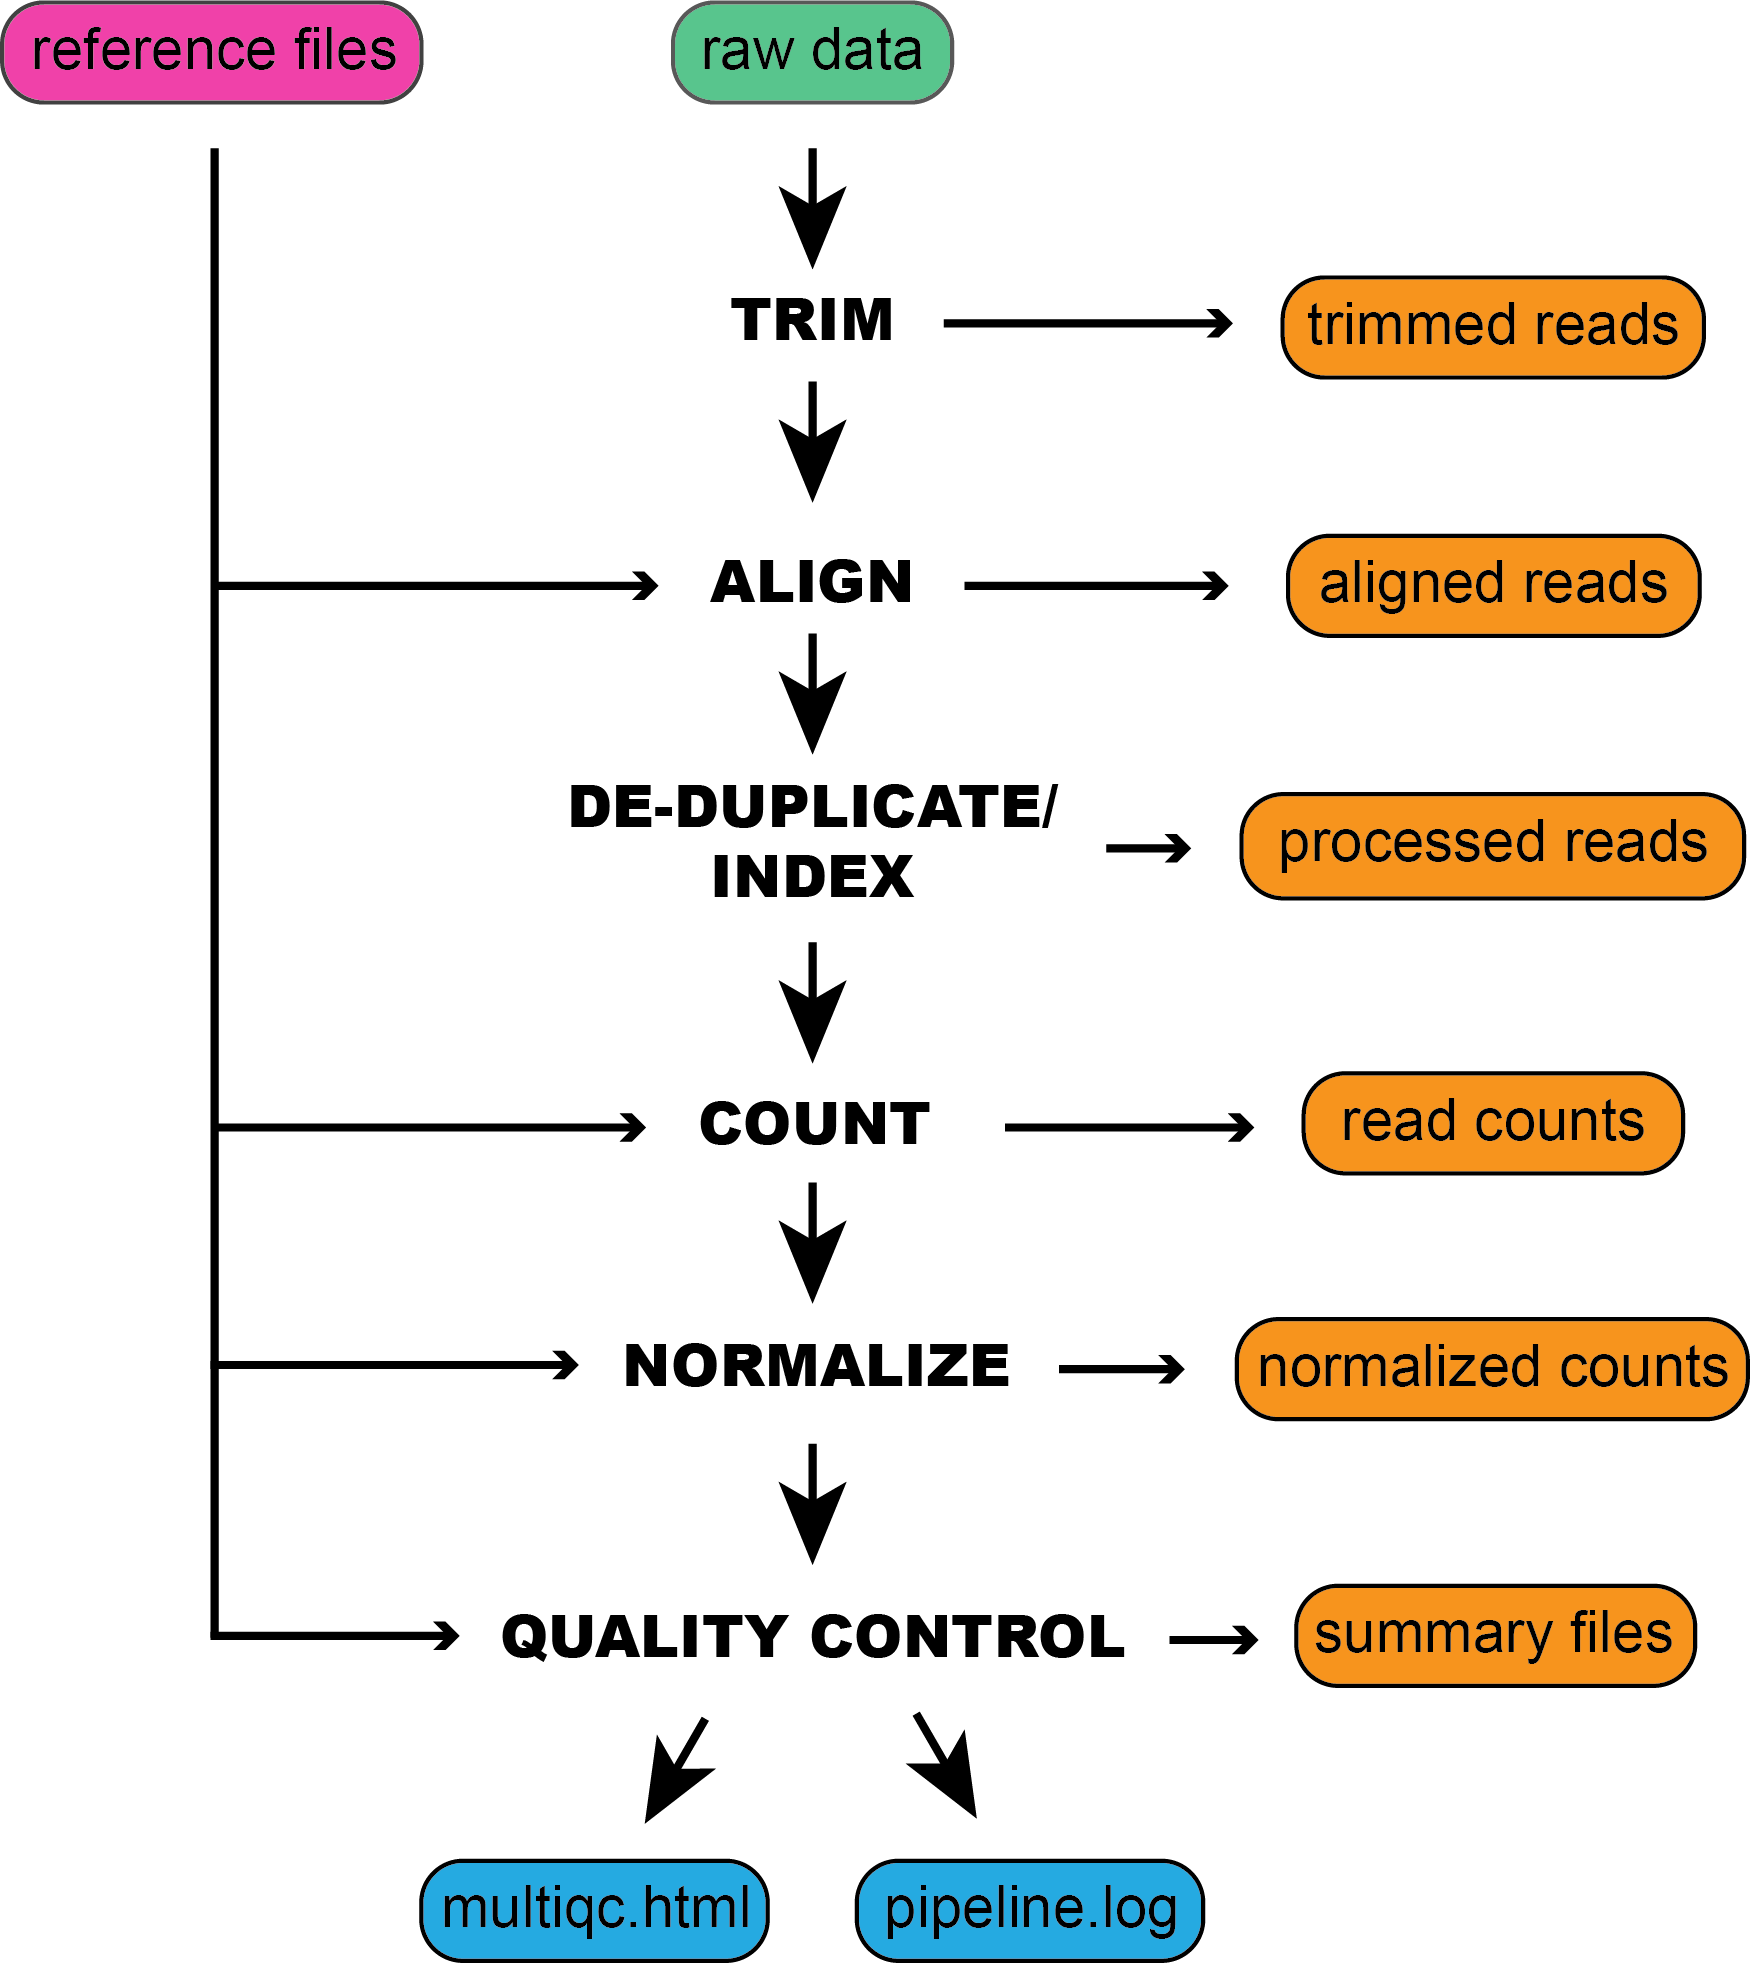
\includegraphics[width=120mm]{figures/xpresspipe_overview.png}
  \caption{\textbf{An example schematic of the inputs required by XPRESSpipe and organization of the outputs.}}
  \label{fig:outputs}
\end{figure}


\subsection{XPRESSplot}
Further analysis of ribosome profiling or RNA-seq data is handled within XPRESSplot. XPRESSplot is a Python library of analysis and plotting tools that builds upon existing packages, such as Matplotlib \cite{matplotlib} and Seaborn \cite{seaborn} to generate flexible, specific analyses and creates plots frequently used by biological researchers that can each be executed in a single line of code rather than tens to hundreds. Additionally, many included features are currently available in an R or other programming language package but not in a Python package. Brief summaries of key components of this package, as well as descriptions of new or more automated tools are provided below and methods are discussed in subsequent sections. We refer the reader to the documentation (https://xpressplot.readthedocs.io/en/latest) for more detailed instructions for other features in the toolkit. Although XPRESSplot is designed for handling transcriptomics datasets, it is also capable in many cases of handling other -omics datasets, such as microarrays, proteomics, or metabolomics.

\subsubsection{Input Data}
Generally, two inputs are required for all functions within XPRESSplot:

\begin{enumerate}
  \item \textbf{Expression Matrix}: It is assumed the input data matrix = \textit{i} * \textit{j} where \textit{i} (rows) are samples and \textit{j} (columns) are genes or other relative measurement points.
  \item \textbf{Metagene Table}: It is assumed the metagene table is a two column, header-less data matrix where column 0 is the sample ID (as specified in \textit{j} of the expression matrix) and column 1 is the sample group (for example, wild-type or treatment).
\end{enumerate}

\subsubsection{Normalization}
RNA-seq experiments can be normalized by the user using the reads-per-million (RPM), Reads-per-kilobase-million (RPKM) or Fragments-per-kilobase-million (FPKM), or transcripts per million (TPM) methods, as outlined in Equations 1-4 in the Methods \cite{evans_briefbio}. Other normalizations, such as mean centering of \textit{i} features (i.e. genes or other analytes) by sklearn's preprocessing module \cite{scikit_learn} are also available. Count thresholds can also be set to remove genes from an analysis that may be less reliable due to poor ability to be sequenced.

\subsubsection{Analyzing Data}

Although a litany of analysis tools are included in XPRESSplot package as of the time of writing, we will focus on tools unique to this Python library or that are particularly useful and refer the reader to the documentation for further details and examples of additional analysis features.

\subsubsection{Principal Components Analysis}
Principal components analysis (PCA) for the data matrix is computed using Python's SciKit-Learn package \cite{scikit_learn} and desired principal components are plotted in a scatter plot via the Matplotlib \cite{matplotlib} and Seaborn \cite{seaborn} packages. The XPRESSplot PCA module, as in many other analysis modules within XPRESSplot, samples are color-coded for easy visualization of sample groups. Confidence intervals are plotted over the scatterplot using NumPy \cite{numpy1, numpy2}, a feature lacking from Pythonic PCA packages.

\subsubsection{Volcano Plot}
Volcano plots are an efficient method for plotting the magnitude, direction, and significance of changes in expression or other data types between two conditions with multiple replicates each. By providing the categorical names for samples of two conditions in the metadata matrix, XPRESSplot will automate the calculation and plotting of this method. When plotting gene expression values, the RNA-seq-specific volcano plot method should be used which requires a DESeq2-output data table as input. This is essential as RNA-seq datasets follow a negative-binomial distribution rather than a normal distribution \cite{deseq2}. For other uses, such as for proteomics or metabolomics datasets where the data is normally distributed, the general volcano plot method can be used, which will average the  measurements for each analyte between the two conditions and the log\textsubscript{2}(fold change) is calculated. Additionally, for each gene, the P-value between the two conditions is calculated using SciPy's Individual T-test function \cite{scipy}. The log\textsubscript{2}(fold change) and -log\textsubscript{10}(P-value) is then plotted for each gene between the two conditions. Additional features available are the ability to plot threshold lines, highlight subsets of genes within the plot, and label specific genes by name.



\subsection{Validation}
In order to evaluate the ability of XPRESSpipe to provide the user with reliable results, we processed publicly available raw sequence files using this automated pipeline. We chose to highlight one ribosome profiling dataset to showcase the utility of XPRESSpipe for rapidly extracting potentially interesting biological insights from sequence data. We additionally chose a small validation subset of TCGA samples, processed their raw read data through XPRESSpipe, and compared the counts to the TCGA-processed count tables corresponding to each sample.

\subsubsection{New Insights from Published Ribosome Profiling Data}
The integrated stress response (ISR) is a signaling mechanism used by cells and organisms in response to a variety of cellular stresses \cite{harding_isr}. Although acute ISR activation is essential for cells to properly respond to stresses, long periods of sustained ISR activity can be damaging. These prolonged episodes lead to a variety of diseases, including many that result in neurological decline \cite{isr_disease}. A recently discovered small-molecule inhibitor of the ISR, ISRIB, has been demonstrated to have therapeutic potential and relative lack of side-effects. Interestingly, ISRIB can suppress the damaging chronic low activation of the ISR, while it does not interfere with a cytoprotective acute, high-grade ISR. It has also been shown to be neuroprotective in mouse models of traumatic brain injury \cite{isrib_activation, isrib_structure, isrib_riboseq, isrib_neuroprotective, isrib_neuroprotective2, isrib_neuroprotective3, isrib_neuroprotective4}. \par

A recent study (data available under Gene Expression Omnibus accession number GSE65778) utilized ribosome profiling to better define the mechanisms of ISRIB action on the ISR, modeled by 1-hour tunicamycin (Tm) treatment in HEK293T cells \cite{isrib_riboseq}. AA key finding of this study is that a specific subset of stress-related transcription factors mRNAs display increased translational efficiency (TE) compared to untreated cells during tunicamycin-induced ISR. However, when cells were co-treated with tunicamycin and ISRIB, the TE of these stress-related mRNAs showed no significant increase, which indicates that ISRIB is able to counteract the translational changes caused by the ISR. In order to showcase the utility of XPRESSpipe in re-analyzing ribosome profiling and sequencing datasets, we re-processed and analyzed this dataset using the more current \textit{in silico} techniques included in the XPRESSpipe package to further query the translational mechanisms of the ISR and ISRIB. Compared to the raw count data made available in the original manuscript, samples showed generally comparable read alignments between the two analytical regimes (all Spearman R values 0.90-0.92) (Figure \ref{fig:figure2}A, \ref{fig:supplement2}). This is in spite of the fact that the methods section of the original publication outlines the use of now outdated software, such as TopHat2 \cite{tophat2}, which has a documented higher false positive alignment rate compared to the current state-of-the-art tool, STAR \cite{alignment_benchmark, star} and likely accounts for the higher alignment rate of certain genes. Additional points of difference may include that this alignment and quantification within XPRESSpipe uses the most recent human transcriptome reference, which no doubt contains modifications to annotated canonical transcripts and so forth when compared to the version available when the original study was published. All XPRESSpipe-processed biological replicate samples exhibited high correlation between read alignments (all Spearman R values 0.98-0.99) (Figure \ref{fig:figure2}B). While these differences in processing between the original publication and XPRESSpipe methods may not create immense differences in output, key biology may be missed. The analysis that follows is exploratory and only meant to suggest putative targets identifiable by re-analyzing pre-existing, publicly available data. \par

\begin{figure}
\centering
  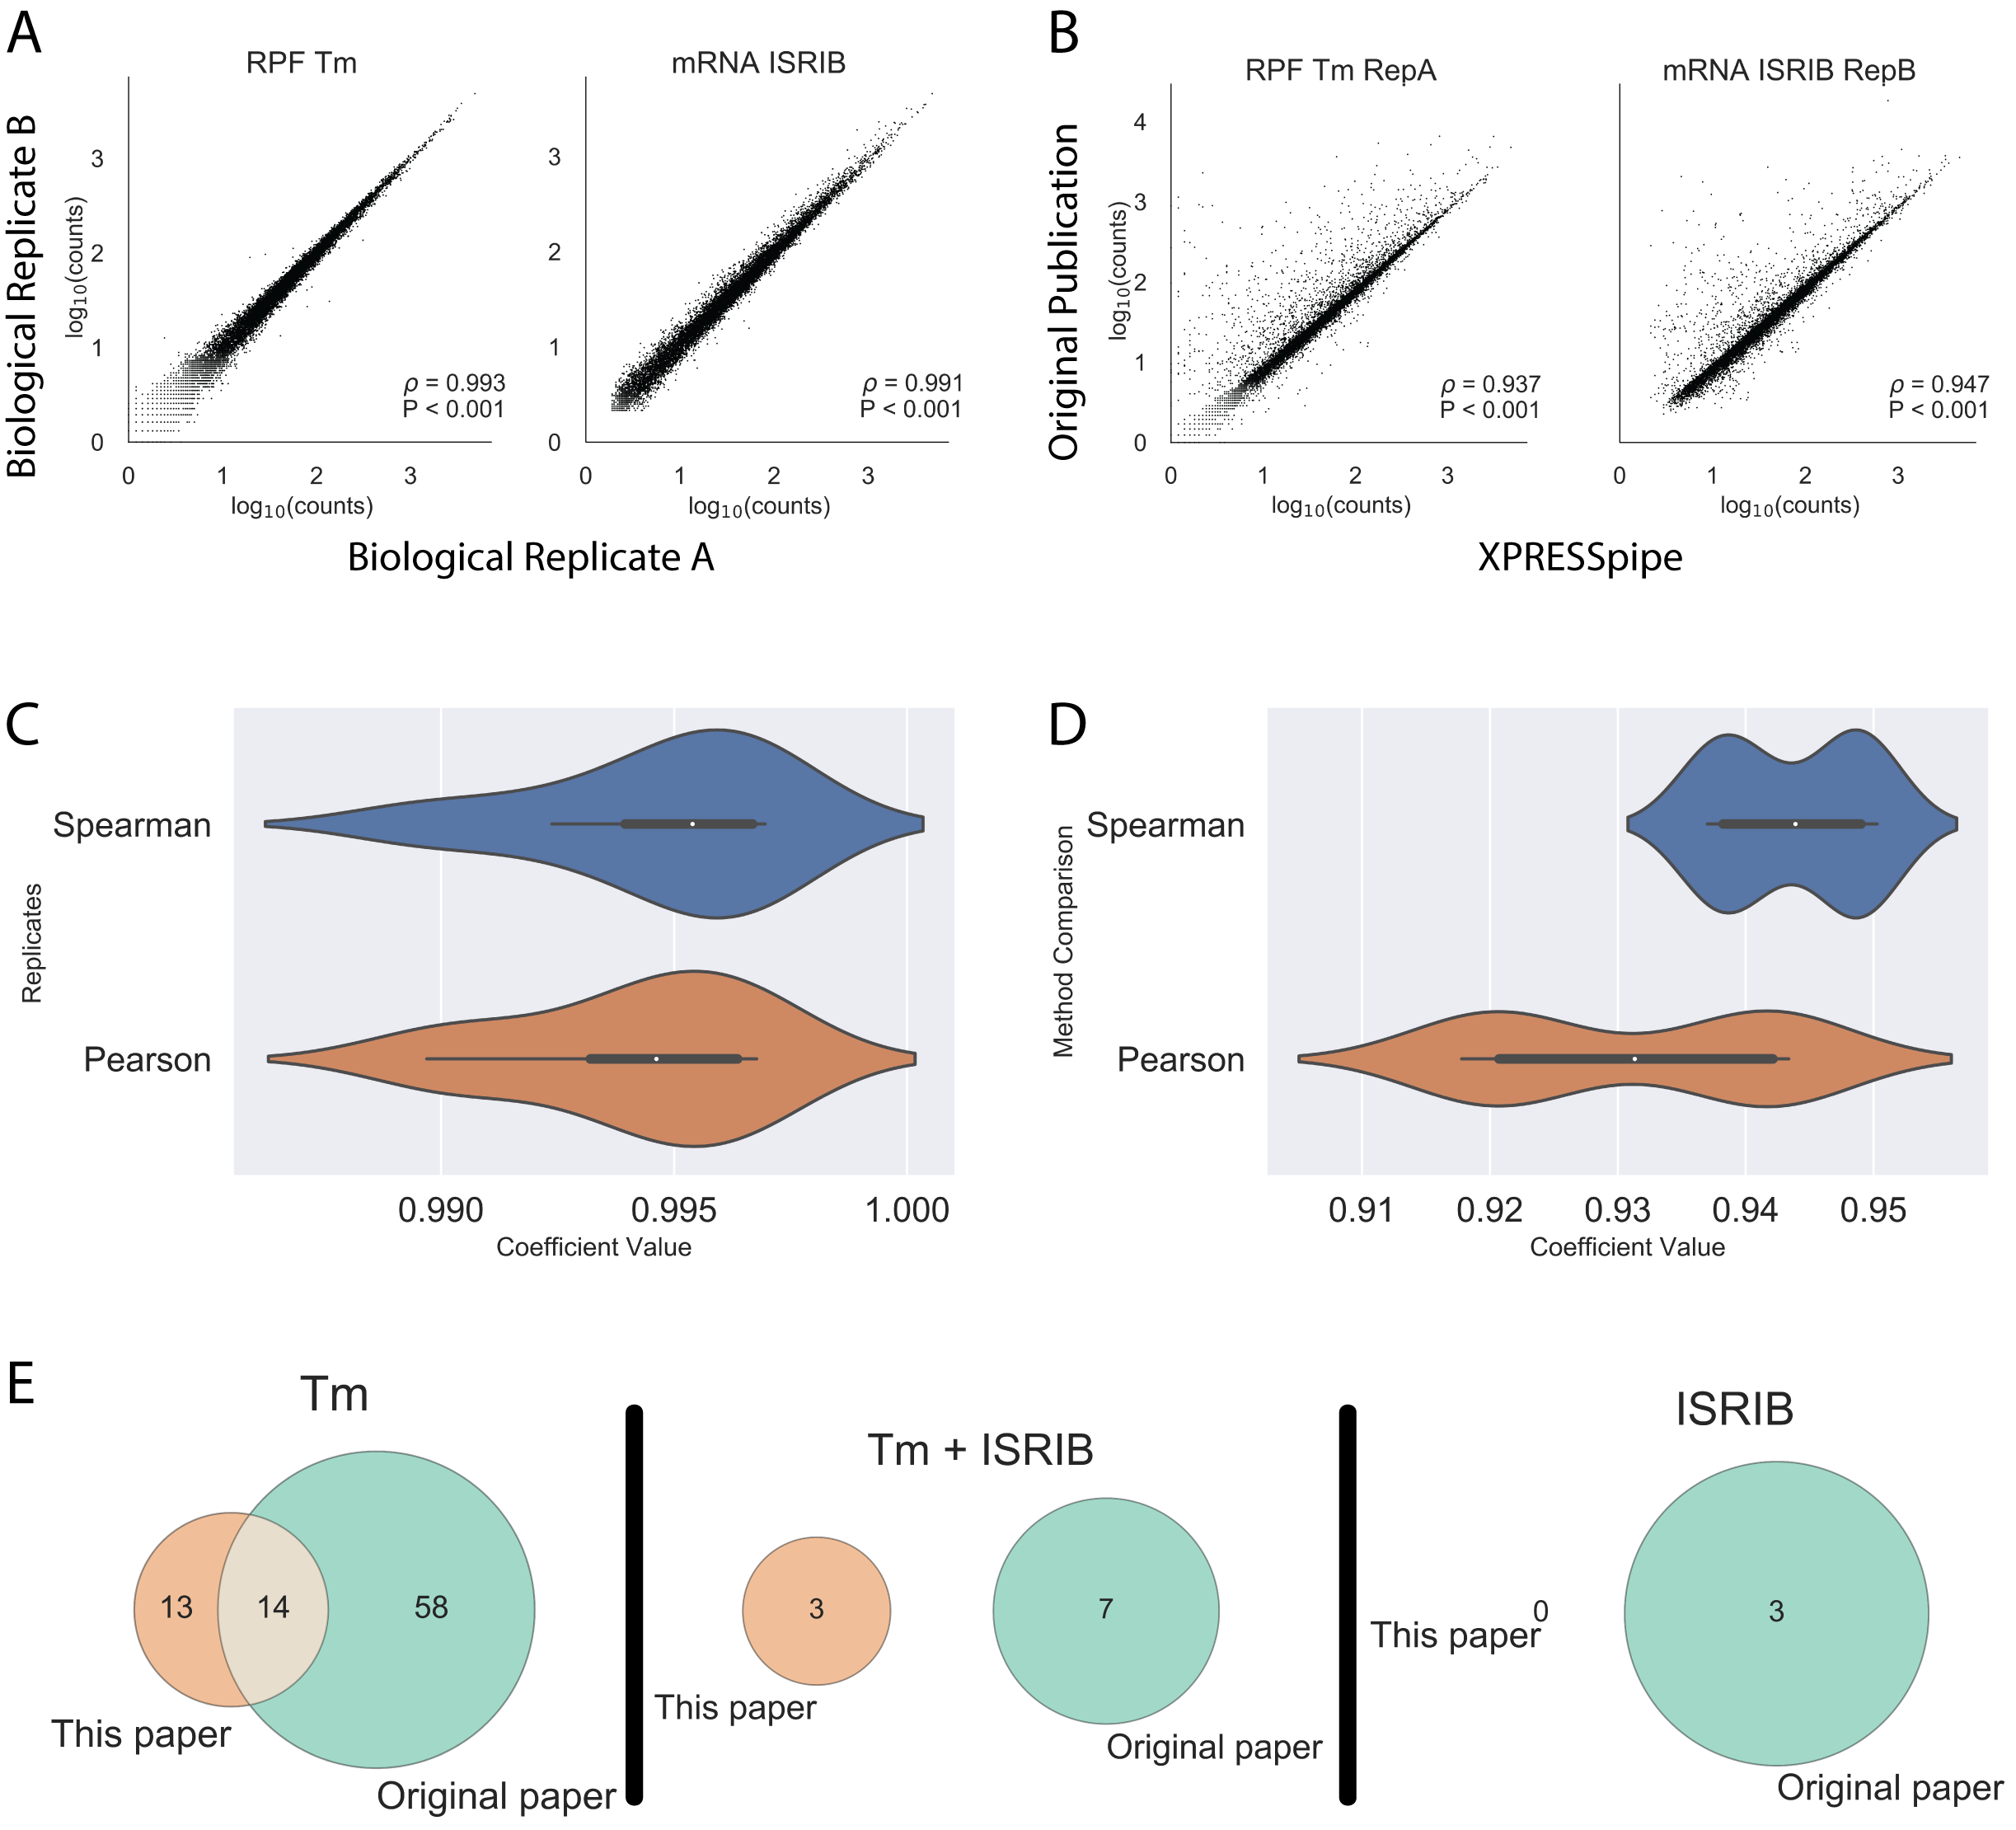
\includegraphics[width=160mm]{figures/xpresspipe_figure2.png}
  \caption{\textbf{Comparison between processed data produced by XPRESSpipe and original study.} A) Comparison of read alignments between count data from the original study and the same raw data processed and quantified by XPRESSpipe. B) Comparison of biological replicate read counts processed by XPRESSpipe. RPF, ribosome-protected fragments. Tm, tunicamycin. All R values reported are Spearman R values.}
  \label{fig:figure2}
\end{figure}

\begin{figure}
\centering
  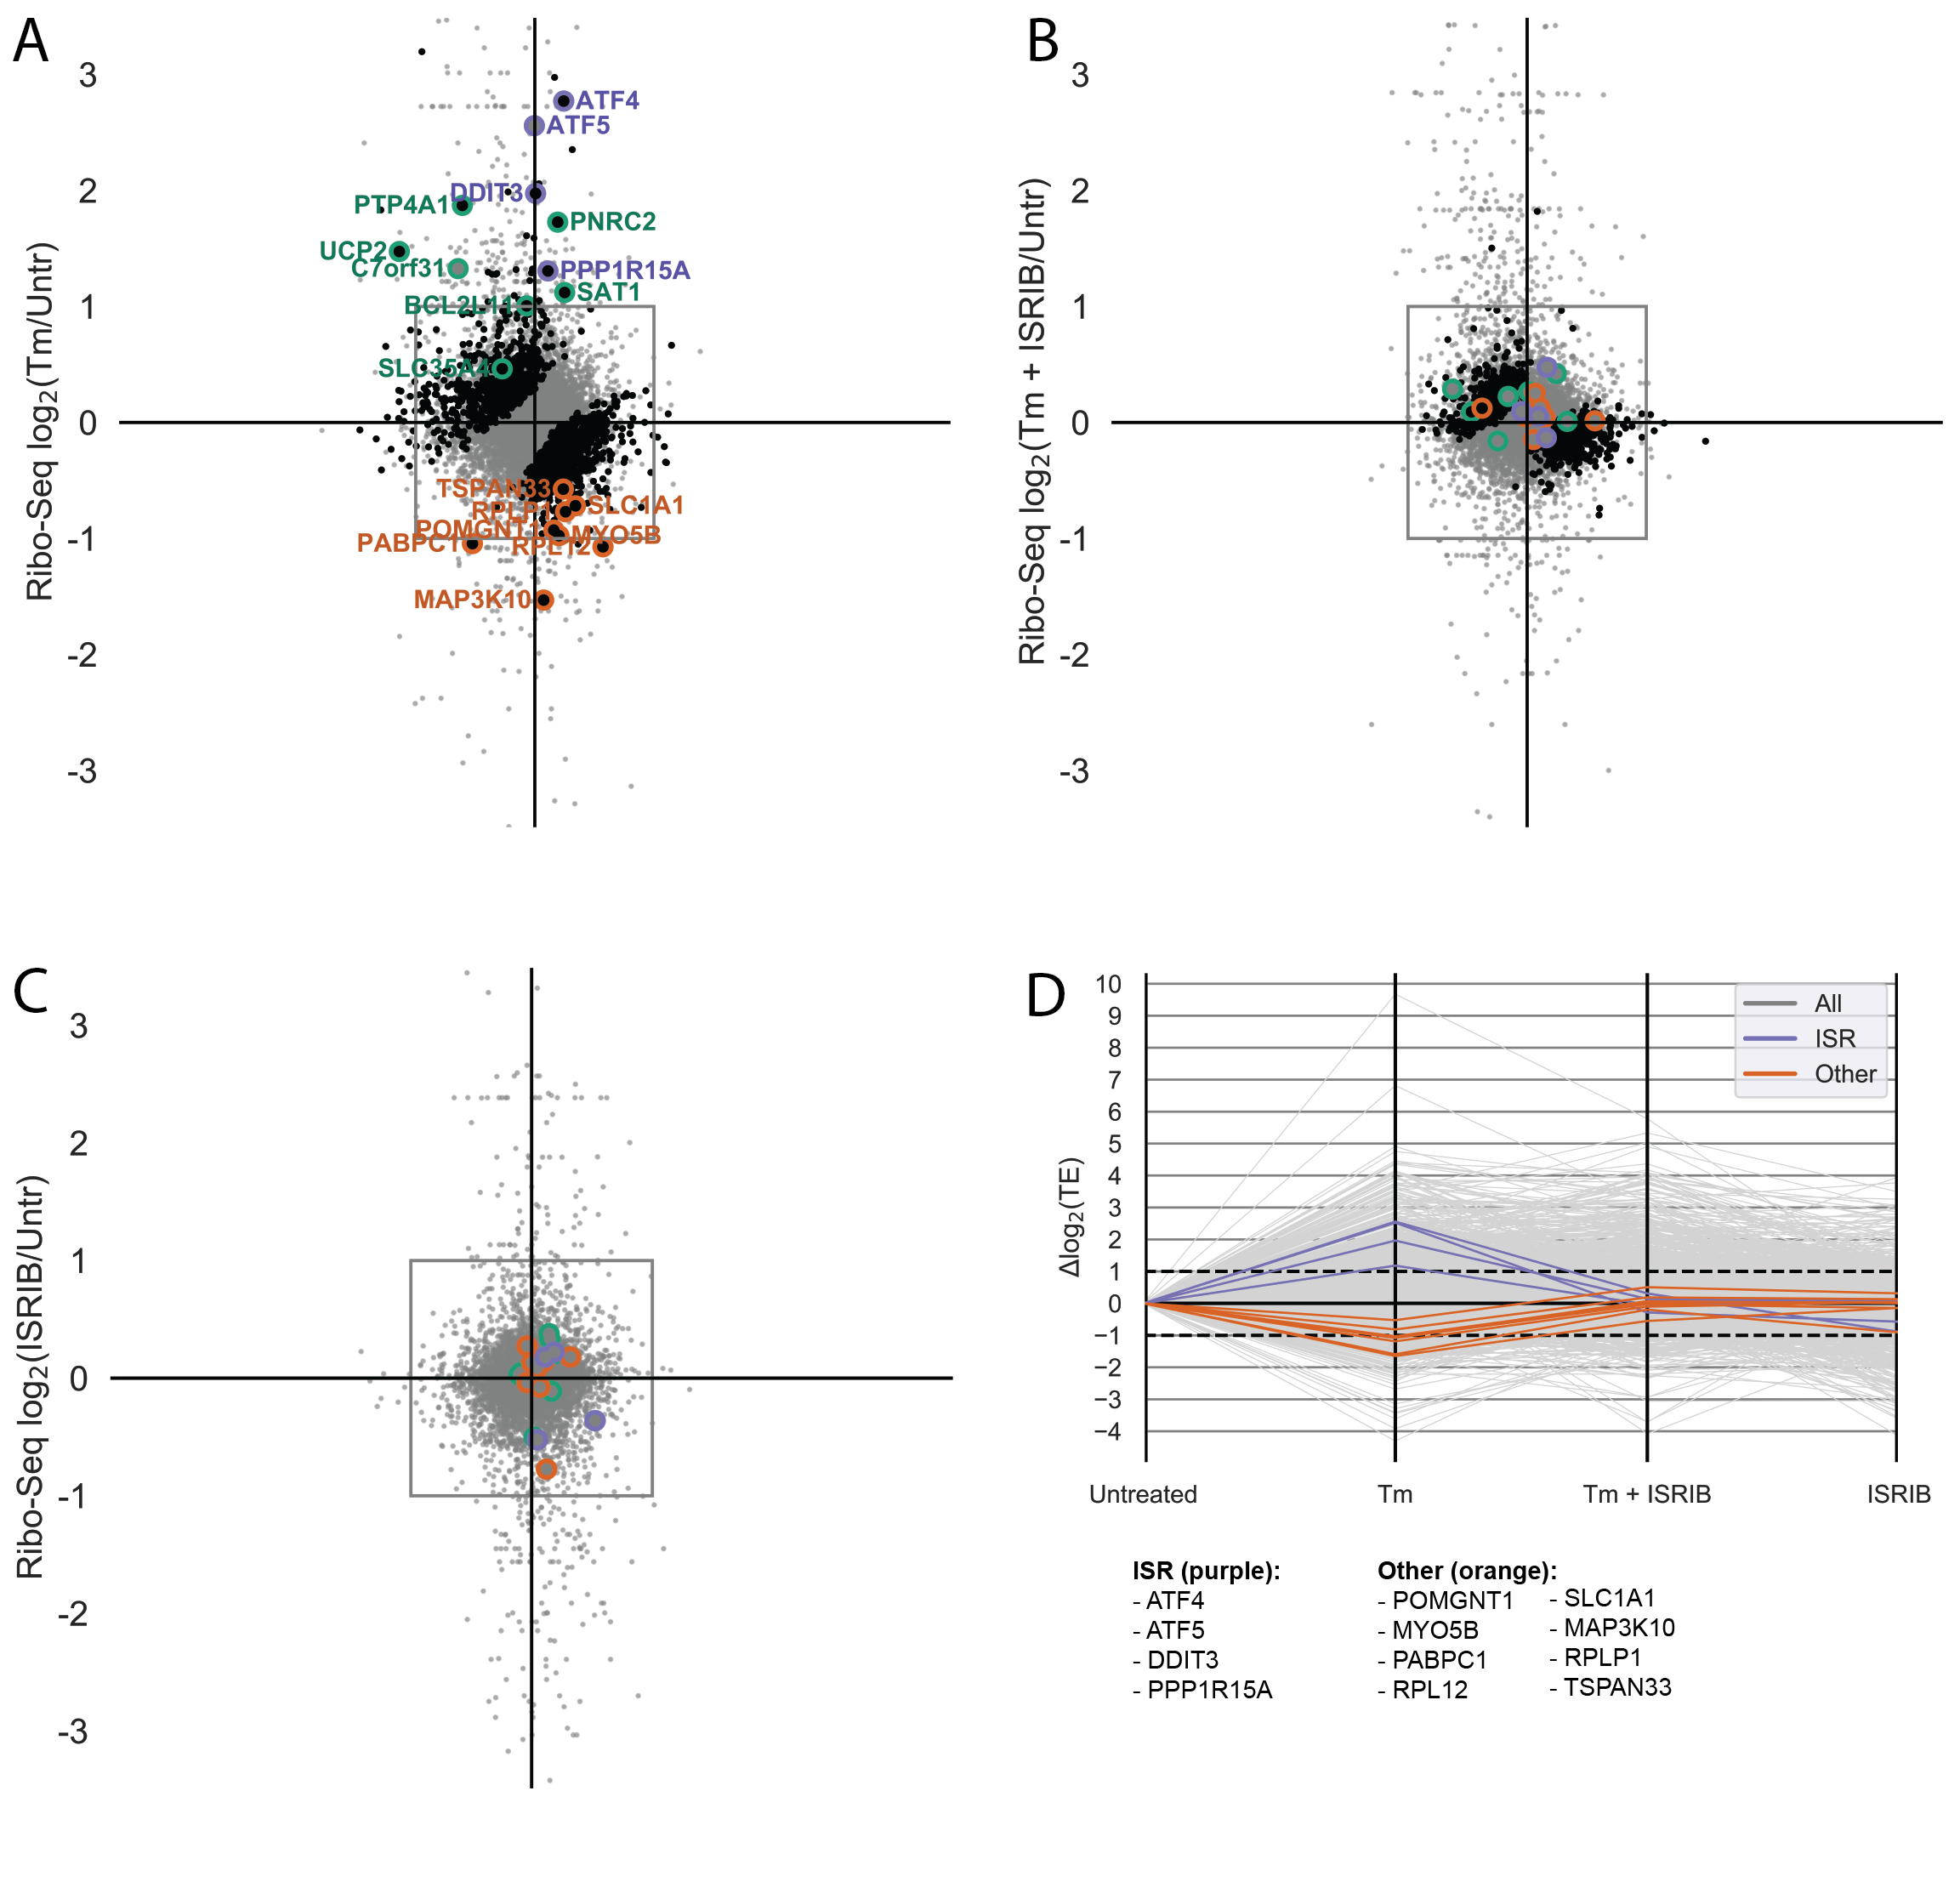
\includegraphics[width=180mm]{figures/xpresspipe_figure3.png}
  \caption{\textbf{Analysis of previously published ISR TE data using XPRESSpipe.} A-C) Fold change for each drug condition compared to untreated for the ribosome profiling and RNA-seq data. Purple, ISR canonical targets highlighted in the original study. Green, genes with uORFs affected by ISR as highlighted in the original study. Black, genes with statistically significant changes. Grey, all genes. Changes in ribo-seq and mRNA-seq were calculated using DESeq2. TE was calculated using DESeq2 (see methods). Points falling outside of the plotted range are not included. D) Changes in log\textsubscript{2}(TE) for each drug condition compared to untreated control. Grey, all genes. Purple, ISR targets identified in the original study. Orange, genes fitting a strict thresholding paradigm to identify genes that display a 2-fold or greater increase in TE in Tm + ISRIB treatment compared to Tm treatment.}
  \label{fig:figure3}
\end{figure}

Similar canonical targets of translational regulation during ISR were identified in the XPRESSpipe-processed data compared to the original study. These targets include ATF4, ATF5, PPP1R15A, and DDIT3 (Figure \ref{fig:figure3}A-C, highlighted in purple) \cite{isrib_riboseq}. Of note, the fold-change in ribosome occupancy of ATF4 (6.74) from XPRESSpipe-processed samples closely mirrored the estimate from the original publication (6.44). Other targets highlighted in the original study \cite{isrib_riboseq}, such as ATF5, PPP1R15A, and DDIT3 also demonstrated increases in their ribosome occupancy fold-changes as compared to the original processing (XPRESSpipe: 5.82, 2.46, and 3.27; respectively. Original: 7.50, 2.70, and 3.89; respectively) (Figure \ref{fig:figure3}A). Similar to the originally processed data, all of these changes in ribosome occupancy return to untreated levels during Tm + ISRIB co-treatment (Figure \ref{fig:figure3}B). Additional ISR uORF targets highlighted in the study (highlighted in green in Figure \ref{fig:figure3}A-C) also mirrored changes in translational and transcriptional regulation across the conditions from the original study. \par

In the original study, translationally down-regulated genes were reported but not discussed. However, re-analyzing these data with the updated XPRESSpipe methodology identifies genes not identified in the original publication that may play a role in the neurodegenerative effects of ISR and the neuroprotective properties of ISRIB \cite{isrib_neuroprotective,isrib_neuroprotective2,isrib_neuroprotective3,isrib_neuroprotective4} and that were not identified as significantly down-regulated in the original analysis. For example, one might expect putative mechanisms related to ISR neurodegeneration and recovery that are translationally-regulated to be significantly translationally down-regulated during ISR and show recovery towards an untreated state during the ISR + ISRIB treatment. Using this paradigm as a guide, we identified eleven genes following this pattern of translational regulation, as listed in Table \ref{tab:targets} (descriptions sourced from https://www.genecards.org/, https://www.ncbi.nlm.nih.gov/gene/, and https://www.uniprot.org/uniprot/; annotations accessed 27 Jun 2019) (Figure \ref{fig:figure3}D). These ISRIB-responsive targets act as interesting putative targets for further validation in a model better mirroring the neurological environment than HEK-293T cells.

Further analysis of these potential hits is strengthened by investigating read pile-ups along these genes in IGV \cite{igv} (Figure \ref{fig:supplement3}). This is an important consideration as the use of CircLigase in the library preparation can bias certain molecules' incorporation in sequencing libraries \cite{circligase_bias}. Distributed footprint coverage is observed across transcripts for all highlighted genes; however, while certain samples appear to be down-regulated in these plots, specific regulation should not be inferred from this information as it has not been sample-normalized. Four out of the eleven hits passing this strict pattern threshold have annotated neurological functions, and another 2 have neurological phenotype annotations. This provides further context to these particular hits for future follow-up for whether these genes contribute to the neurodegenerative phenotypes observed during ISR and the ability of ISRIB to be neuroprotective during ISR.

For example, SLC1A1 is a glutamate transporter vital for neurotransmission and maintaining glutamate homeostasis. Deficits in this transporter can lead to neurotoxic levels of glutamate within a cell. This transporter is densely expressed throughout the brain \cite{slc1a1_neurotoxic}. Down-regulation of SLC1A1 has already been implicated in diseases such as neurodegenerative diseases caused by mutations in the eukaryotic translation initiation factor 2B subunit epsilon (eIF2B5) \cite{eif2b_neuroprotective}. ISR operates by a similar mechanism, where eIF2$\alpha$ is phosphorylated and general changes in protein translation are observed \cite{isrib_riboseq, isrib_structure}. This suggests that SLC1A1 abundance control by translation initiation factors is key in an array of neurological conditions and may be partially responsible for the neurodegeneration observed in prolonged ISR conditions. ISRIB's neuroprotective descriptions may, therefore, stem from a recovery of SLC1A1 levels to wild-type levels, which in turn helps regulate glutamate levels. Glutamate transporters, like SLC1A1, have even been implicated in preventing neurotrauma within the first few minutes of insult \cite{slc1a1_neurotoxic}. Within 1 hour of ISR-induction in the published ribosome profiling study we are analyzing \cite{isrib_riboseq}, there was a large decrease in translation efficiency of SLC1A1, suggesting that a rapid disruption or recovery in a vital transporter may play a role in these neurodegenerative and neuroprotective properties.

\begin{table}[!]
    \centering
\captionof{table}{\textbf{Translationally down-regulated genes during acute Tm treatment and recovered regulation during Tm + ISRIB treatment.}}
\begin{tabular}{p{2.5cm}p{15.5cm}}
 \textbf{Gene Name} & \textbf{Relevant Description} \\
 \hline
 POMGNT1 & Participates in O-mannosyl glycosylation. Mutations have been associated with muscle-eye-brain diseases and congenital muscular dystrophies. Expressed especially in astrocytes, as well as in immature and mature neurons. Expressed across brain stem cells. \\
 \hline
 MYO5B & May be involved in plasma membrane recycling. Identified in the original ISRIB study. No related neurological annotations. \\
 \hline
 PABPC1 & Promotes ribosome recruitment and translation initiation. May contribute to mRNA stability. No related neurological annotations. \\
 \hline
 RPL12 & Ribosomal subunit. No related neurological annotations. \\
 \hline
 SLC1A1 & Dense expression in substantia nigra, red nucleus, hippocampus, and cerebral cortical layers. Member of high-affinity glutamate transporter. In the brain, crucial for terminating postsynaptic action of the neurotransmitter glutamate. Responsible for maintaining glutamate concentrations below neurotoxic levels. \\
 \hline
 MAP3K10 & Functions in JNK signaling, reportedly involved in nerve growth factor induces neuronal apoptosis. Expressed in the cerebral cortex. Activates NEUROD1, which promotes neuronal differentiation. \\
 \hline
 RPLP1 & Ribosome subunit. Evidence for stem cell and embryonic expression in the cerebral cortex. \\
 \hline
 TSPAN33 & Plays a role in normal erythropoiesis and regulates maturation and trafficking of ADAM10, a metalloprotease. Negatively regulates Notch activity by way of its regulation of ADAM10. Notch signaling is vital to neurogenesis. \\
 \label{tab:targets}
\end{tabular}
\end{table}


\subsubsection{Performance Validation Using TCGA Data}
To validate the general design and reliability of the XPRESSpipe pipeline, we processed raw TCGA sequence data using XPRESSpipe and compared the output count values to those publicly available through TCGA (https://portal.gdc.cancer.gov/). Spearman R values for the selected samples ranged from 0.95-0.96 (Figure \ref{fig:figure4}), indicating XPRESSpipe performs with similar accuracy to the TCGA RNA-seq processing standards. \par

The differences in reported counts can be accounted for by a couple of key differences. For example, the XPRESSpipe-processed files are aligned to the Homo sapiens GRChv96 reference transcriptome, while the original count data are aligned to the GRChv79 reference transcriptome. As seen in Figure \ref{fig:supplement4}A, the use of a different transcriptome reference can result in large differences in the final quantified data for a number of genes. To wit, in the four years between these versions, significant advances have been made in our understanding of transcribed regions of the human genome. Between versions 95 and 96 alone (version 95 published 24 Nov 2018, version 96 published 13 Mar 2019), approximately 32,259 records were added (quantified by difference in line numbers between the files). \par

Another source of differences in data processing stems from the use of only Ensembl canonical transcripts only during quantification. TCGA-processed data used an un-modified transcriptome reference file (all transcripts); therefore, the use of this modified (longest transcript only) GTF will produce varied quantification for some genes as quantifications are constrained to a single transcript version of a given gene and a read will not be quantified if mapping to an exon not used by the canonical transcript. Even using XPRESSpipe settings closest to the TCGA pipeline and using the same genome and transcriptome version resulted in some variation (Figure \ref{fig:supplement4}A, plot enclosed in maroon). By performing a closer analysis of these differences, it is clear that virtually all genes exhibiting differences between the processing methods are pseudogenes (Figure \ref{fig:supplement4}B), with the TCGA pipeline quantifying more pseudogenes, which can be indicitive of an aligner's inability to recognize these reads as multimapping to both the original gene and pseudogene.  \par


\begin{figure}
\centering
  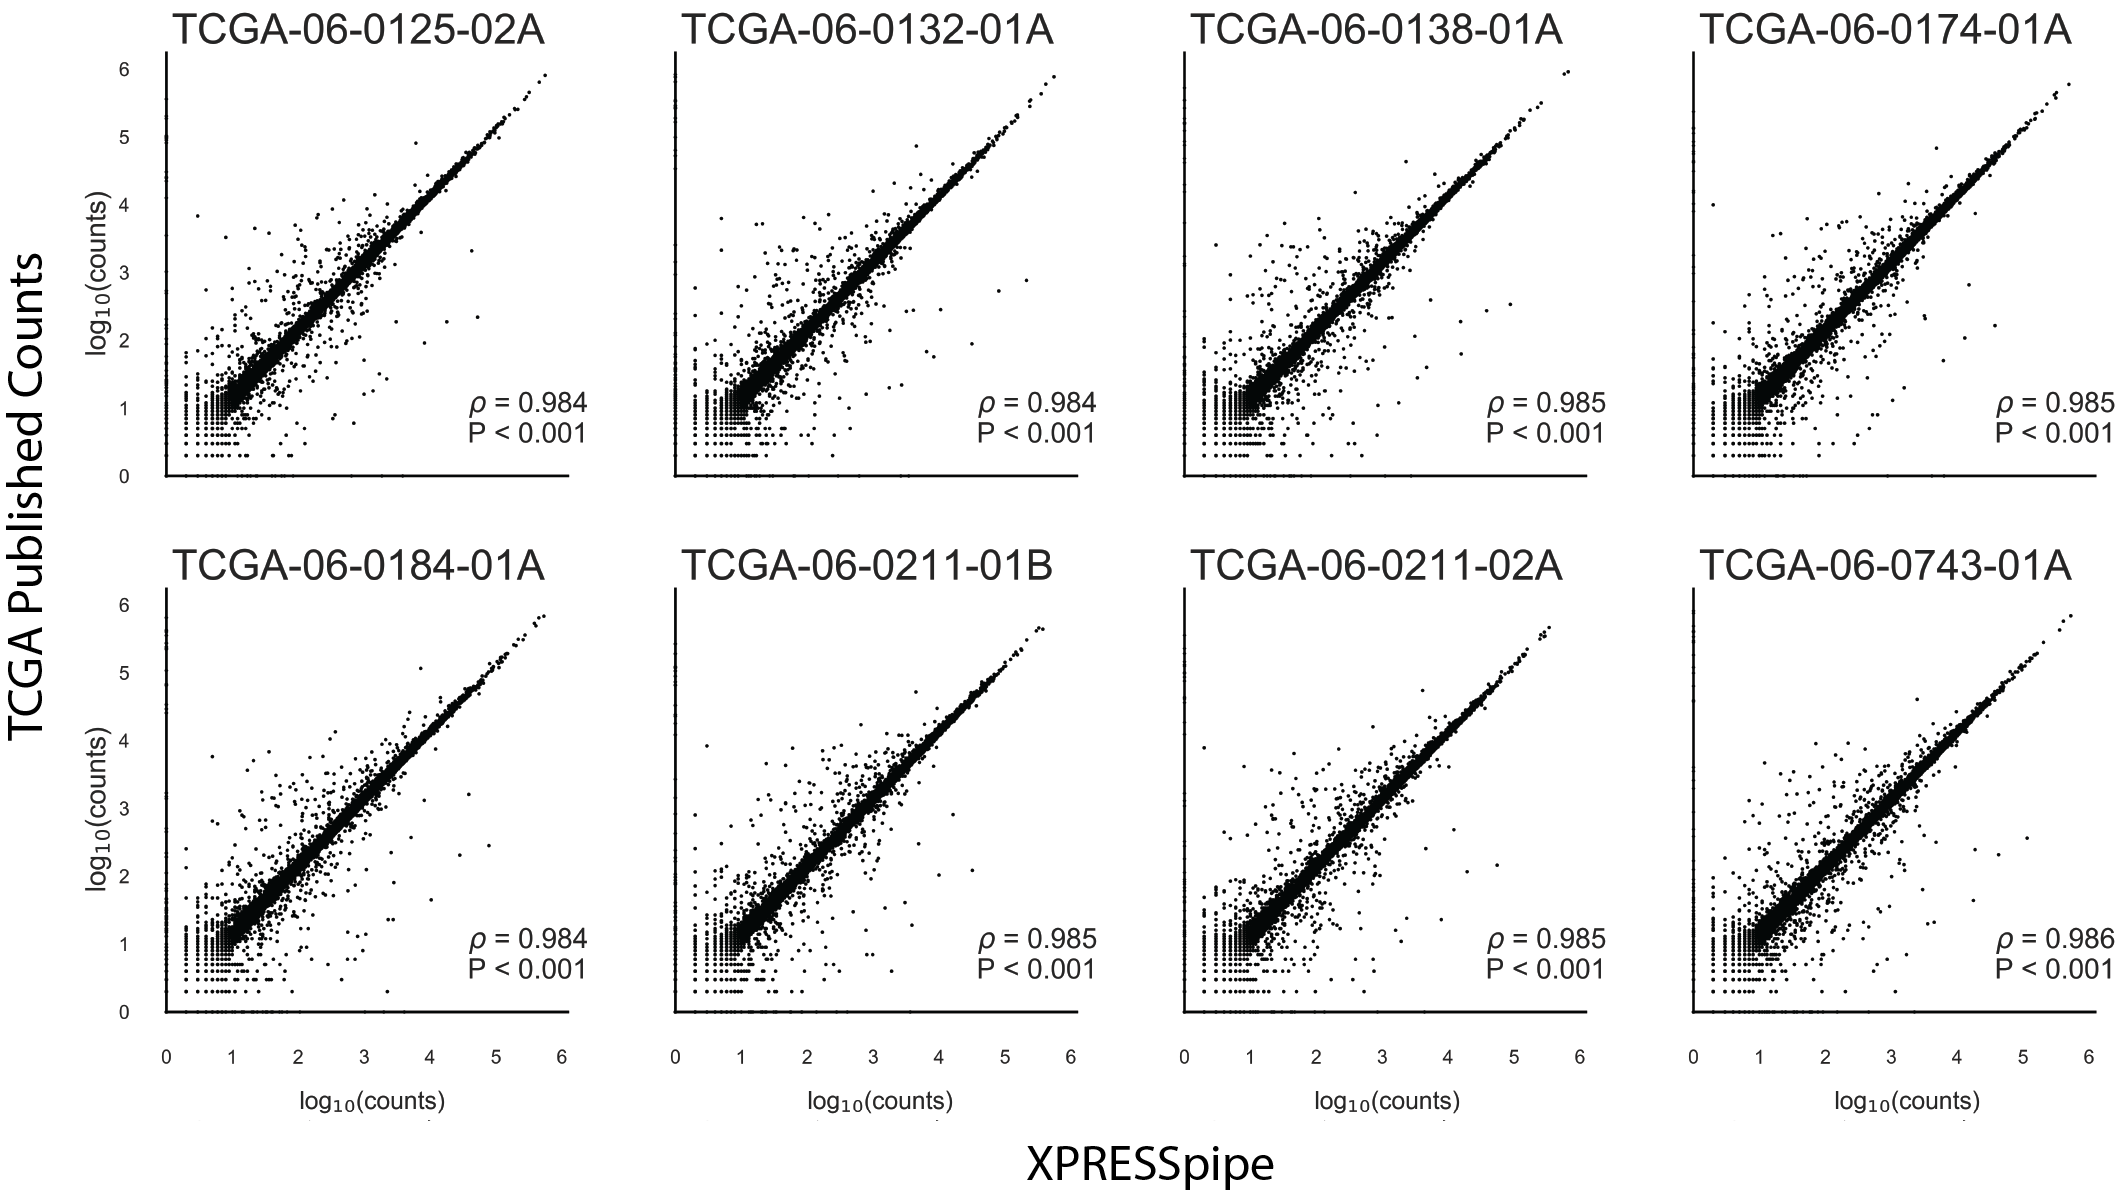
\includegraphics[width=180mm]{figures/xpresspipe_figure4.png}
  \caption{\textbf{Pipeline validation using publicly available TCGA count data.} Correlations were calculated between publicly available count data from TCGA samples and the XPRESSpipe on the sequence count data. Note: All R values reported are Spearman R values. All axes are log\textsubscript{10}(counts).}
  \label{fig:figure4}
\end{figure}


\subsubsection{Cost Analysis}
XPRESSpipe functions can be computationally intensive and thus, super-computing resources are recommended. Many universities provide super-computing resources to their staff and students; however, in cases where these resources are not available, servers such as Amazon Web Services (AWS) (https://aws.amazon.com/) can be used to process sequencing data using XPRESSpipe. The ISRIB ribosome profiling dataset discussed above contained a total of 32 raw sequence files. Table \ref{tab:chpc_performance} outlines runtime statistics, providing an example of the time required to process a dataset.

% UPDATE BEFORE SUBMISSION ONCE QUALITY CONTROL STABLE AND CHECK CONVERSIONS\
--------------->UPDATE<-----------------------
\begin{table}[!]
    \centering
\captionof{table}{\textbf{XPRESSpipe processing statistics for dataset GSE65778.}}
\begin{tabular}{p{5cm}p{3cm}}
\textbf{Metric} & \textbf{Value} \\
\hline
 Elapsed Real Time & 09h32m58s \\
 \hline
 Total CPU Time & 1d10h11m42s \\
 \hline
 Allocated CPUs & 16 \\
 \hline
 Allocated Memory per Node & 62.50GB \\
 \hline
 Maximum RAM of all tasks & 62.60GB \\
 \label{tab:chpc_performance}
\end{tabular}
\end{table}

Based on these metrics, if high-performance computing services are not locally available, processing could be performed on a platform such as Amazon Web Services to process the data for relatively little money. For a comparable run, storage cost would amount to around 14 USD/month on Amazon S3 storage and compute cost for a similar computational node for the given elapsed time would cost approximately 7.50 USD using Amazon EC2 On-Demand m5.4xlarge node (however, significantly reduced rates are available if using Spot instances or by using the free tier; calculations were performed 28 Jun 2019). \par


\section{Discussion}
We have described a new software suite, XPRESSyourself, which includes a set of tools to aid in expression data processing and analysis. Although RNA-seq technologies are becoming more and more established, standardized computational protocols are much less established for some applications. This is problematic when individuals or groups may not be using the most up-to-date methods or be aware of particular biases or measures of quality control required to produce a reliable, high-quality sequencing study. XPRESSpipe handles these issues through continuous curation of benchmarked software tools and by simplifying the required user input. It also outputs all necessary quality control metrics so that the user can quickly assess quality and identify any systematic problems or technical biases that may be present in their samples. \par

An additional problem XPRESSpipe addresses is the incorrect use of these software tools, which is especially important for those coming from a non-computational background. XPRESSyourself will dissolve this barrier-to-entry for most users so that they can process and analyze their data immediately upon receipt of the raw data and only requires simple programming knowledge covered by simple video walkthroughs, example scripts, and interactive command builders. \par

A particular strongpoint of XPRESSyourself is that it consolidates and streamlines many tools specific to ribosome profiling processing and analysis. This includes producing GTF files with $5'$ and $3'$ truncated CDS annotations, rRNA probe design for subtractive hybridization of abundant rRNA contaminants, and quality-control analyses to report on ribosome footprint periodicity and metagene coverage. \par

We demonstrated the utility of the XPRESSyourself toolkit by re-analyzing a publicly available ribosome profiling dataset. From this analysis, we identified putative hits that may contribute to the neurodegenerative effects of integrated stress response (ISR) and how the molecule ISRIB may be acting on these genes to confer neuroprotection. This additionally highlights the importance of re-analyzing older datasets with more current methods, as improved analysis methodologies and updated organism genetic references may result in new interpretations and hypotheses. XPRESSyourself will enable individuals and labs to process and analyze their own data, which will often result in quicker turnaround of experiments as well as monetary savings. XPRESSyourself will also put missing or incomplete computational tools required for ribosome profiling and RNA-seq into the hands of the average user. Additionally, usage inclusion of detailed log reports, summaries of software dependencies used during runtime, and containerized versions of the pipeline where dependencies are archived and self-contained will aid in reproducibility and make transparent methods easy to incorporate into associated publications. \par


\section{Conclusions}
With the adoption of this flexible pipeline, the field of high-throughput sequencing, particularly within ribosome profiling, can continue to standardize the processing protocol for sequencing data and eliminate some of the variability that comes from using a variety of software packages for various steps during read processing. Additionally, XPRESSpipe consolidates various tools used by the ribosome profiling and RNA-seq communities. With these tools, such as the GTF modification sub-module, genome reference formatting and curation is automated and accessible to the public. Further, by using this pipeline on publicly available data, we highlight XPRESSpipe's utility in being able to re-process publicly available data or personal data to uncover novel biological patterns quickly. Adoption of this tool will aid scientists with quickly accessing their data.


\section{Materials and Methods}
Methods described in this manuscript apply to the software packages at the time of writing. To obtain the most current methods, please refer to the documentation or source code for a given module.

\subsection{Software Dependencies}
A list of dependencies required for XPRESSpipe at the time of writing is listed in Table \ref{Tab:software_pipe}. Dependencies for XPRESSplot at the time of writing are listed in Table \ref{Tab:software_plot}.

% Software dependencies table
\begin{table}[!]
    \centering
\captionof{table}{\textbf{Summary of dependency software, accession location, and purpose in the XPRESSpipe package.}}
\begin{tabular}{p{2.4cm}p{7.5cm}p{3cm}}
 \textbf{Package} & \textbf{Purpose} & \textbf{Reference} \\
 \hline
 Python & Primary language & \\
 \hline
 R & Language used for some statistical modules & \\
 \hline
 fastp & Read pre-processing & \cite{fastp} \\
 \hline
 STAR & Reference curation and read alignment & \cite{star} \\
 \hline
 samtools & Alignment file manipulation & \cite{samtools} \\
 \hline
 bedtools & Alignment file manipulation & \cite{bedtools} \\
 \hline
 Cufflinks & Read quantification (primary) & \cite{cufflinks} \\
 \hline
 HTSeq & Read quantification & \cite{htseq} \\
 \hline
 FastQC & Quality Control & \cite{fastqc} \\
 \hline
 MultiQC & Quality Control & \cite{multiqc} \\
 \hline
 pandas & Data manipulation & \cite{pandas} \\
 \hline
 numpy & Data manipulation & \cite{numpy1, numpy2} \\
 \hline
 scipy & Data manipulation & \cite{scipy} \\
 \hline
 sklearn & Data manipulation & \cite{sklearn} \\
 \hline
 matplotlib & Plotting & \cite{matplotlib} \\
 \hline
 XPRESSplot & Normalization and matrix manipulation & This paper \\
 \hline
 dupRadar & Perform library complexity calculations & \cite{dupradar} \\
 \hline
 DESeq2 & Perform differential expression analysis & \cite{deseq2} \\
 \label{Tab:software_pipe}
\end{tabular}
\end{table}

% Software dependencies table
\begin{table}[!]
    \centering
\captionof{table}{\textbf{Summary of dependency software, accession location, and purpose in the XPRESSplot package.}}
\begin{tabular}{p{2.4cm}p{7.5cm}p{3cm}}
 \textbf{Package} & \textbf{Purpose} & \textbf{Reference} \\
 \hline
 Python & Primary language & \\
 \hline
 R & Language used for some statistical modules & \\
 \hline
 Pandas & Data manipulation & \cite{pandas} \\
 \hline
 NumPy & Data manipulation & \cite{numpy1, numpy2} \\
 \hline
 SciPy & Data manipulation & \cite{scipy} \\
 \hline
 Matplotlib & Plotting & \cite{matplotlib} \\
 \hline
 Seaborn & Plotting & \cite{seaborn} \\
 \hline
 Plotly & Interactive plotting & \cite{plotly} \\
 \hline
 scikit-learn & Data manipulation & \cite{sklearn} \\
 \hline
 SVA & Perform batch correction for known effects with the ComBat function & \cite{sva} \\
 \label{Tab:software_plot}
 \end{tabular}
\end{table}

\subsection{GTF Modification}
In order to parallelize GTF modification, a GTF file is split into approximately equal chunks equal to the specified number of threads. To avoid an incomplete gene record being included in a chunk, a given chunk end point is determined by calculating the size of the GTF, dividing by the number of threads, and advancing one chunk size forward in line number, then advancing line by line until the last line of the current gene record. If creating the last chunk, the end of the chunk is automatically the last line of the GTF record. \par

Ensembl canonical transcripts are determined according to the Ensembl glossary definition of a canonical transcript. For cases where a tie-breaker exists with equal priority transcripts, the longest is chosen. When there are more than one of these equal priority transcripts of the same length exist, the first listed record is retained. Exon or CDS lengths are calculated by taking the sum of each exon or CDS, not including intron or other space in the calculation. \par

Protein-coding records are retained by performing a simple string search on the attribute column of the GTF file for the ``protein\_coding" annotation. \par

Truncation of records is performed by identifying the $5'$ and $3'$ end of each transcript and modifying the given coordinates to reflect the given truncation amounts. Suggested truncation amounts are 45 nt from the $5'$ end and 15 nt from the $3'$ end, which are set as the default truncatin amount parameters for the function and do not need to be modified unless the user desires \cite{ingolia_meth}. As a given CDS portion of a given exon may be less than a truncation amount, the function will recursively search CDS by CDS per transcript until the full truncation amount is fully trimmed. Any record smaller than the sum of the $5'$ and $3'$ truncation amounts is removed from the output file. \par

\subsection{GTF Flattened Record}
Flattened transcriptome references are created for meta-analysis modules by providing a GTF. This curation operates in a similar manner to the methods employed by general GTF modification; however, only exon or CDS records are retained with other minimal key information (i.e. strandedness). These records are then divided into a multidimensional array, where each parent is a chromosome. \par

\subsection{Normalization}
Equations 1-4 reflect the design of the normalization functions within XPRESSplot, where \textit{g} is gene \textit{n}, \textit{ge} is cumulative exon space for gene \textit{n}, \textit{r} is total reads, \textit{f} is total fragments, and \textit{l} is length.

  \begin{equation}
    RPM\textsubscript{g} = \frac{1e6 \cdot r\textsubscript{\textit{ge}}}{\sum_{g=1}^{n} r\textsubscript{\textit{ge}}}
  \end{equation}
  \begin{equation}
    RPKM\textsubscript{g} = \frac{1e6 \cdot r\textsubscript{\textit{ge}}}{(\sum_{g=1}^{n} r\textsubscript{\textit{ge}}) \cdot \textit{l} \textsubscript{\textit{ge}}}
  \end{equation}
  \begin{equation}
    FPKM\textsubscript{g} = \frac{1e6 \cdot f\textsubscript{\textit{ge}}}{(\sum_{g=1}^{n} f\textsubscript{\textit{ge}}) \cdot \textit{l} \textsubscript{\textit{ge}}}
  \end{equation}
  \begin{equation}
    TPM\textsubscript{g} = \frac{1e6 \cdot r\textsubscript{\textit{ge}}}{(\sum_{g=1}^{n} (\frac{r\textsubscript{\textit{ge}}}{l\textsubscript{\textit{ge}}})) \cdot \textit{l} \textsubscript{\textit{ge}}}
  \end{equation}


\subsection{Quality Control Summary Plotting}
Summary plots are created using Pandas \cite{pandas} and Matplotlib \cite{matplotlib}. Kernel density plots for library complexity analyses are created using NumPy \cite{numpy1, numpy2} and SciPy's \texttt{gaussian\_kde} function \cite{scipy}.

\subsection{Metagene Estimation}
Metagene calculations are performed by determining the meta-genomic coordinate \textit{M} for each aligned read, where \textit{L\textsubscript{e}} is the leftmost mapped position of the read (strand agnostic) and \textit{r} is the length of the mapped read. \textit{S} denotes the start coordinate for the transcript and \textit{l\textsubscript{e}} is the cumulative length of all exons for the given transcript. The subscripted \textit{e} indicates the coordinate is relative to exon space (intronic ranges within a transcript do not contribution to total space calculation). Required inputs are an indexed BAM file and an un-modified GTF reference file, which is then curated into its longest-transcript, protein-coding-only flattened form, as discussed above. If a longest-transcript, protein-coding-only modified GTF has already been curated, this can alternatively be provided as input, with which the module will flatten. For each mapped coordinate, the metagene position is calculated as:
\begin{equation}
\textit{M} = \frac{|(L\textsubscript{e}\ +\ \frac{1}{2}r)\ -\ S|\ \cdot\ 100}{\textit{l\textsubscript{e}}}
\end{equation}

In the case where a mapped coordinate falls within multiple genes, a penalty is assigned as:
\begin{equation}
  \textit{c} = \frac{1}{\textit{n}}
\end{equation}
Where \textit{c} is the count score for a given meta-position and \textit{n} is the number of different transcripts a given coordinate mapped. To be counted or factored into the penalty, the meta-position coordinate must fall within exon space.

\subsection{Periodicity}
Ribosome p-site periodicity is calculated using riboWaltz \cite{ribowaltz}. Required inputs are the path to a directory containing transcriptome-aligned BAM files (ending in ``toTranscriptome.out.bam") and the path and file name of the appropriate un-modified GTF.

\subsection{rRNA Probe}
\texttt{rrnaProbe} works on a directory containing FastQC \cite{fastqc} zip compressed files to detect over-represented sequences for each sample. These sequences are then collated to create consensus fragments. One caveat is that FastQC collates on exact matching strings, but these strings, or sequences, can be 1 nt steps from each other and a single rRNA probe could be used to effectively pull out all these sequences. In order to handle this situation, XPRESSpipe will combine these near matches. A rank-ordered list of over-represented fragments within the appropriate length range to target for depletion is then output. A BLAST \cite{blast} search on these consensus sequences intended for probe usage can then be performed to verify the fragment maps to an rRNA sequence and is thus a suitable depletion probe.

\subsection{Confidence Interval Plotting}
Confidence intervals within PCA scatterplots generated by XRESSplot are calculated as follows:

\begin{enumerate}
  \item Compute the covariance of the two principal component arrays, \textit{x} and \textit{y} using the numpy.cov() function.

  \item Compute the eigenvalues and normalized eigenvectors of the covariance matrix using the numpy.linalg.eig() function.

  \item Compute the $\theta$ of the normalized eigenvectors using the numpy.arctan2() function and converting the output from radians to degrees using numpy.deg().

  \item Compute the $\lambda$ of the eigenvalues by taking the square root of the eigenvalues.

  \item Plot the confidence intervals over the scatter plot: The center point of the confidence interval is determined from the means of the \textit{x} and \textit{y} arrays. The angle is set equal to $\theta$. The width of the confidence interval is calculated by
  \[
  \textit{w} = \lambda _{\textit{\scriptsize{x}}}\ \cdot\ \textit{ci}\ \cdot\ 2
  \]
  where \textit{ci} is equal to the corresponding confidence level (i.e. 68\% = 1, 95\% = 2, 99\% = 3). The height is similarly computed by
  \[
  \textit{h} = \lambda _{\textit{\scriptsize{y}}}\ \cdot\ \textit{ci}\ \cdot\ 2
  \]
\end{enumerate}

\subsection{Ribosome Profiling Data Analysis}
Raw data were obtained from GEO (GSE65778). Reference files were taken from Ensembl Human build GRCh38 version 96. All associated figures and analyses can be reproduced using the associated scripts found at https://github.com/XPRESSyourself/manuscript (DOI: XXXXXX). See https://github.com/j-berg/xpressyourself\_manuscript/tree/master/isrib\_analysis/batch\_run\_docs for scripts used to process data. \par

Only gene names in common between the original data file and XPRESSpipe output were used for the method comparisons. Correlation between methods or replicates were calculated using a Spearman rank correlation coefficient, performed using the \texttt{scipy.stats.spearman()} function \cite{spearman_rnaseq}. The associated script can be accessed at https://github.com/j-berg/xpressyourself\_manuscript/blob/master/isrib\_analysis/isrib\_analysis.py. \par

Differential expression analyses were performed using all genes, but with a minimum count of 10 or greater per gene across samples, as recommended by the DESeq2 documentation \cite{deseq2}. Differential expression for ribo-seq and RNA-seq was performed as detailed in the associated scripts (https://github.com/j-berg/xpressyourself\_manuscript/blob/master/isrib\_analysis/isrib\_analysis.py, https://github.com/j-berg/xpressyourself\_manuscript/blob/master/isrib\_analysis/isrib\_de/isrib\_de\_analysis.py, https://github.com/j-berg/xpressyourself\_manuscript/blob/master/isrib\_analysis/isrib\_de/run\_de.sh). For these analysis, the design formula was such that comparisons were designed treated factor level over untreated factor level. Differential expression of translation efficiencies between conditions used the additional incorporation of the ribosome footprint factor level over RNA-seq factor level in the design formula \cite{deseq2,isrib_riboseq,ingolia_meth}. Adjusted p-values in the associated figures were calculated from the differential expression of the translation efficiencies of each gene for a given condition. Those passing an adjusted p-value threshold of less than or equal to 0.1 are highlighted in black. \par

Intron-inclusive gene coverage profiles were generated using IGV \cite{igv}. Interactive scatter plots were generated using Plotly Express \cite{plotly}. \par

\subsection{TCGA Data Analysis}
Raw data and processed TCGA count data was obtained from the TCGA Portal (https://portal.gdc.cancer.gov/) via dbGap controlled access (https://www.ncbi.nlm.nih.gov/gap/). Raw data were processed on a protected high-performance computing environment. Correlations between methods or replicates were calculated using a Spearman rank correlation coefficient, performed using the \texttt{scipy.stats.spearman()} function \cite{spearman_rnaseq}. The associated script can be accessed at https://github.com/j-berg/xpressyourself\_manuscript/blob/master/tcga\_data/tcga\_validation.py. Interactive scatter plots were generated using Plotly Express \cite{plotly} See https://github.com/j-berg/xpressyourself\_manuscript/tree/master/tcga\_data/batch\_process\_info for scripts used to process data. \par


\subsection{Cost Analysis}
Cost analysis was performed by accessing run logs from the high-performance computing cluster and using published AWS prices (https://aws.amazon.com/ec2/pricing/on-demand/, https://aws.amazon.com/s3/pricing/, accessed 28 June 2019) to calculate the relative cost for a similar run.

\section*{List of abbreviations}
AWS - Amazon Web Services,
BAM - Binary Sequence Alignment Map,
BED - Browser Extensible Data,
cDNA - complementary DNA,
CDS - coding region of gene,
ChIP-seq - chromatin immunoprecipitation sequencing,
CPU - central processing unit,
dbGaP - Database of Genotypes and Phenotypes,
DNA - deoxyribonucleic acid,
FPKM - fragments per kilobase of transcript per million,
GEO - Gene Expression Omnibus,
GTF - General Transfer Format,
IGV - Integrative Genomics Viewer,
ISR - integrated stress response,
ISRIB - ISR inhibitor,
nt - nucleotide,
PCA - principal component analysis,
PCR - polymerase chain reaction,
RAM - random access memory,
RNA - ribonucleic acid,
RNA-seq - RNA sequencing
RPKM - reads per kilobase of transcript per million,
RPM - reads per million,
rRNA - ribosomal RNA,
TCGA - The Cancer Genome Atlas,
TE - translation efficiency,
TPM - transcripts per million,
UMI - unique molecular identifier

\section*{Ethics approval and consent to participate}
Protected TCGA data were obtained through dbGaP project number 21674 and utilized according to the associated policies and guidelines.

\section*{Consent for publication}
Protected TCGA data were obtained through dbGaP project number 21674 and utilized according to the associated policies and guidelines.

\section*{Availability of data and materials}
The source code for these packages is perpetually open source and protected under the GPL-3.0 license. The code can be publicly accessed and installed from https://github.com/XPRESSyourself. Updates to the software are version controlled and maintained on GitHub. Jupyter notebooks and video walkthroughs are included on https://github.com/XPRESSyourself for guiding users through the use of the packages. Documentation is hosted on readthedocs \cite{readthedocs} at https://xpresspipe.readthedocs.io/en/latest/ and https://xpressplot.readthedocs.io/en/latest/. The publicly available ribosome profiling data are accessible through GEO series accession number GSE65778. TCGA data are accessible through dbGaP accession number phs000178. Code used to create manuscript figures and analyses can be found at https://github.com/XPRESSyourself/manuscript (DOI: XXXXXX).

\section*{Competing interests}
The authors declare that they have no competing interests.

\section*{Funding}
J.A.B. received support from the National Institute of Diabetes and Digestive and Kidney Diseases (NIDDK) Inter-disciplinary Training Grant T32 Program in Computational Approaches to Diabetes and Metabolism Research, 1T32DK11096601 to Wendy W. Chapman and Simon J. Fisher. A.J.B received support from the National Cancer Institute (NCI) Predoctoral to Postdoctoral Fellow Transition Award, K00CA212445.

\section*{Contributions}
J.A.B. conceptualized and administered the project; performed all investigation, analysis, visualization, and data curation; provisioned resources; acquired funding; and wrote the original draft for this study. J.A.B. and J.R.B. designed and wrote the software. J.A.B., J.T.M., A.J.B., and Y.O. performed software validation. J.A.B., J.R.B., J.T.M., and J.G. and developed the methodology. J.R., A.R.Q., and J.G. supervised the study. All authors were involved in reviewing and editing the manuscript.

\begin{table}[!]
    \centering
\captionof{table}{\textbf{Author ORCIDs}}
\begin{tabular}{p{2.4cm}p{7.5cm}}
 \textbf{Author} & \textbf{ORCID}\\
 \hline
 JAB & 0000-0002-5096-0558 \\
 \hline
 JRB & \\
 \hline
 JTM & \\
 \hline
 AJB & 0000-0003-2273-8922 \\
 \hline
 YO & 0000-0001-9523-1044 \\
 \hline
 ARQ & 0000-0003-1756-0859 \\
 \hline
 JG & 0000-0001-7568-6789 \\
 \hline
 JR & \\
\end{tabular}
\end{table}

\section*{Acknowledgments}
The authors wish to thank Michael T. Howard for helpful discussions concerning ribosome profiling and sequencing analysis. The authors also wish to thank Mark E. Wadsworth, Ryan Miller, and Michael J. Cormier for helpful discussions on pipeline design. They also wish to thank T. Cameron Waller for helpful discussions related to pipeline design and biological analysis. The support and resources from the Center for High-Performance Computing at the University of Utah are gratefully acknowledged. The computational resources used were partially funded by the NIH Shared Instrumentation Grant 1S10OD021644-01A1. The results published here are in whole or part based upon data generated by the TCGA Research Network: https://www.cancer.gov/tcga.

\bibliography{xpressyourself}
\bibliographystyle{Science}

\beginsupplement

\begin{figure}
\centering
  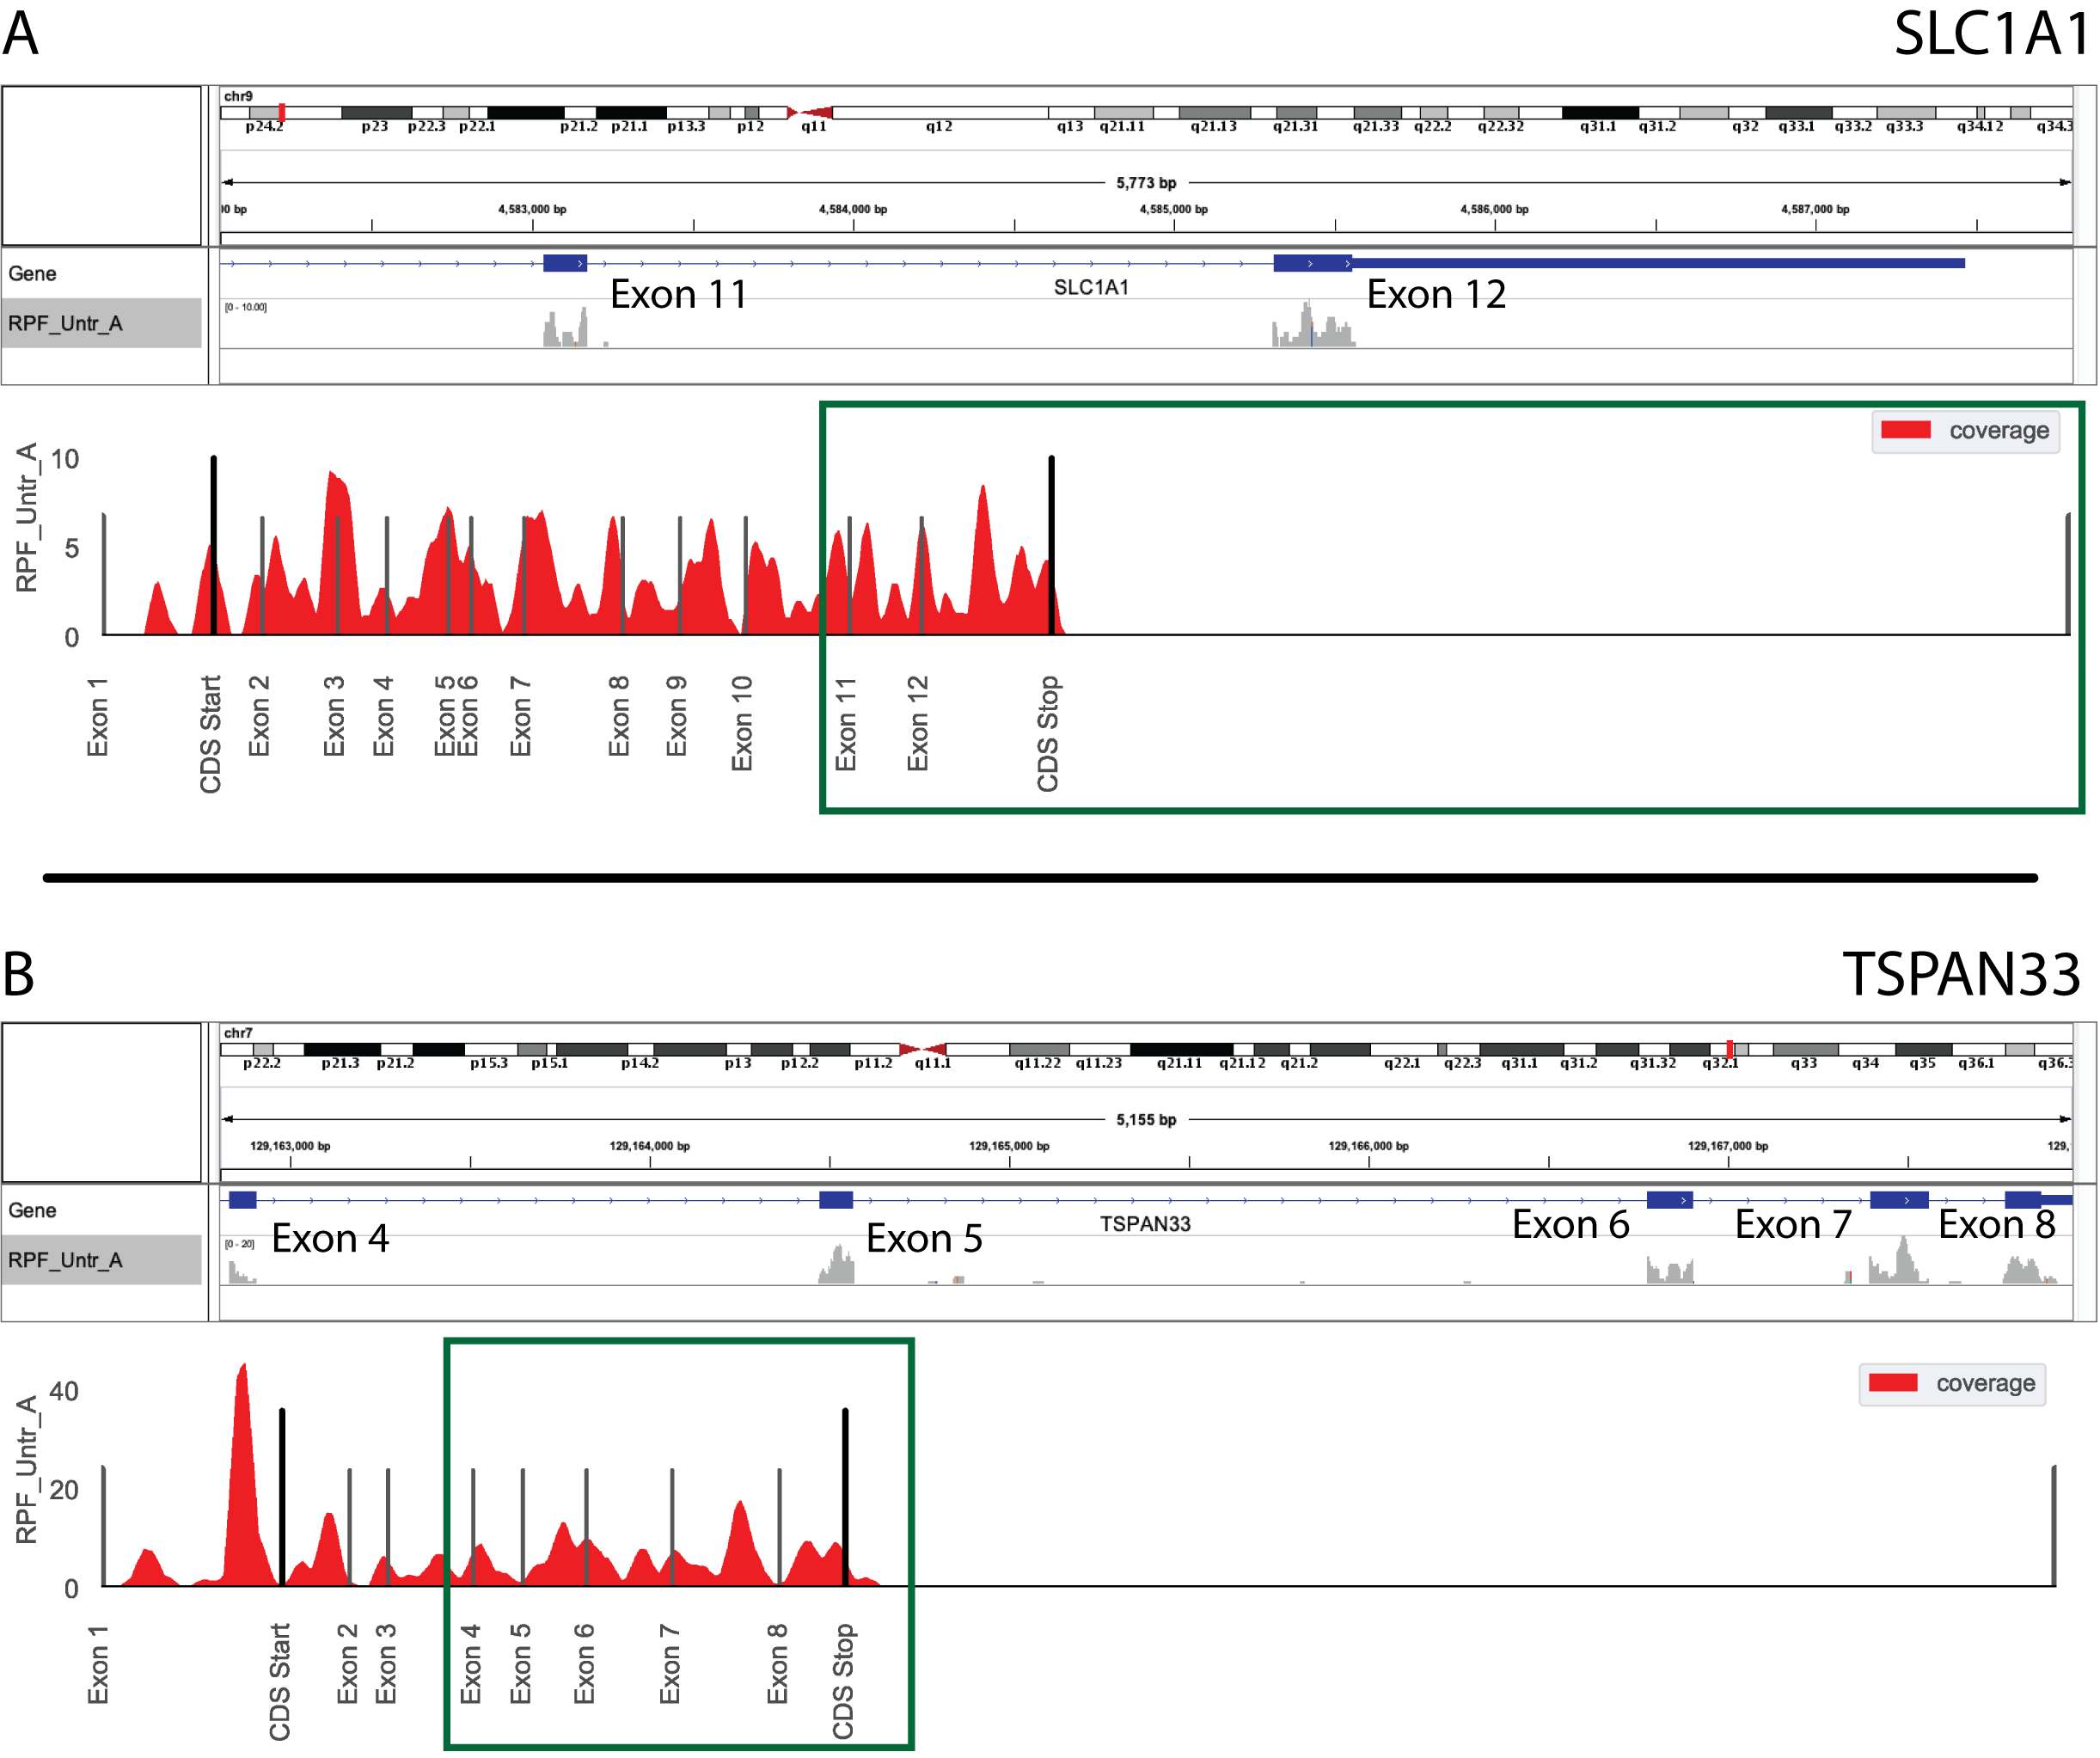
\includegraphics[width=160mm]{figures/xpresspipe_supplement2.png}
  \caption{\textbf{A sampling of the original count data plotted against XPRESSpipe-processed data.} Selected highlighted genes show consistent differences between processing methods.}
  \label{fig:supplement2}
\end{figure}

\begin{figure}
\centering
  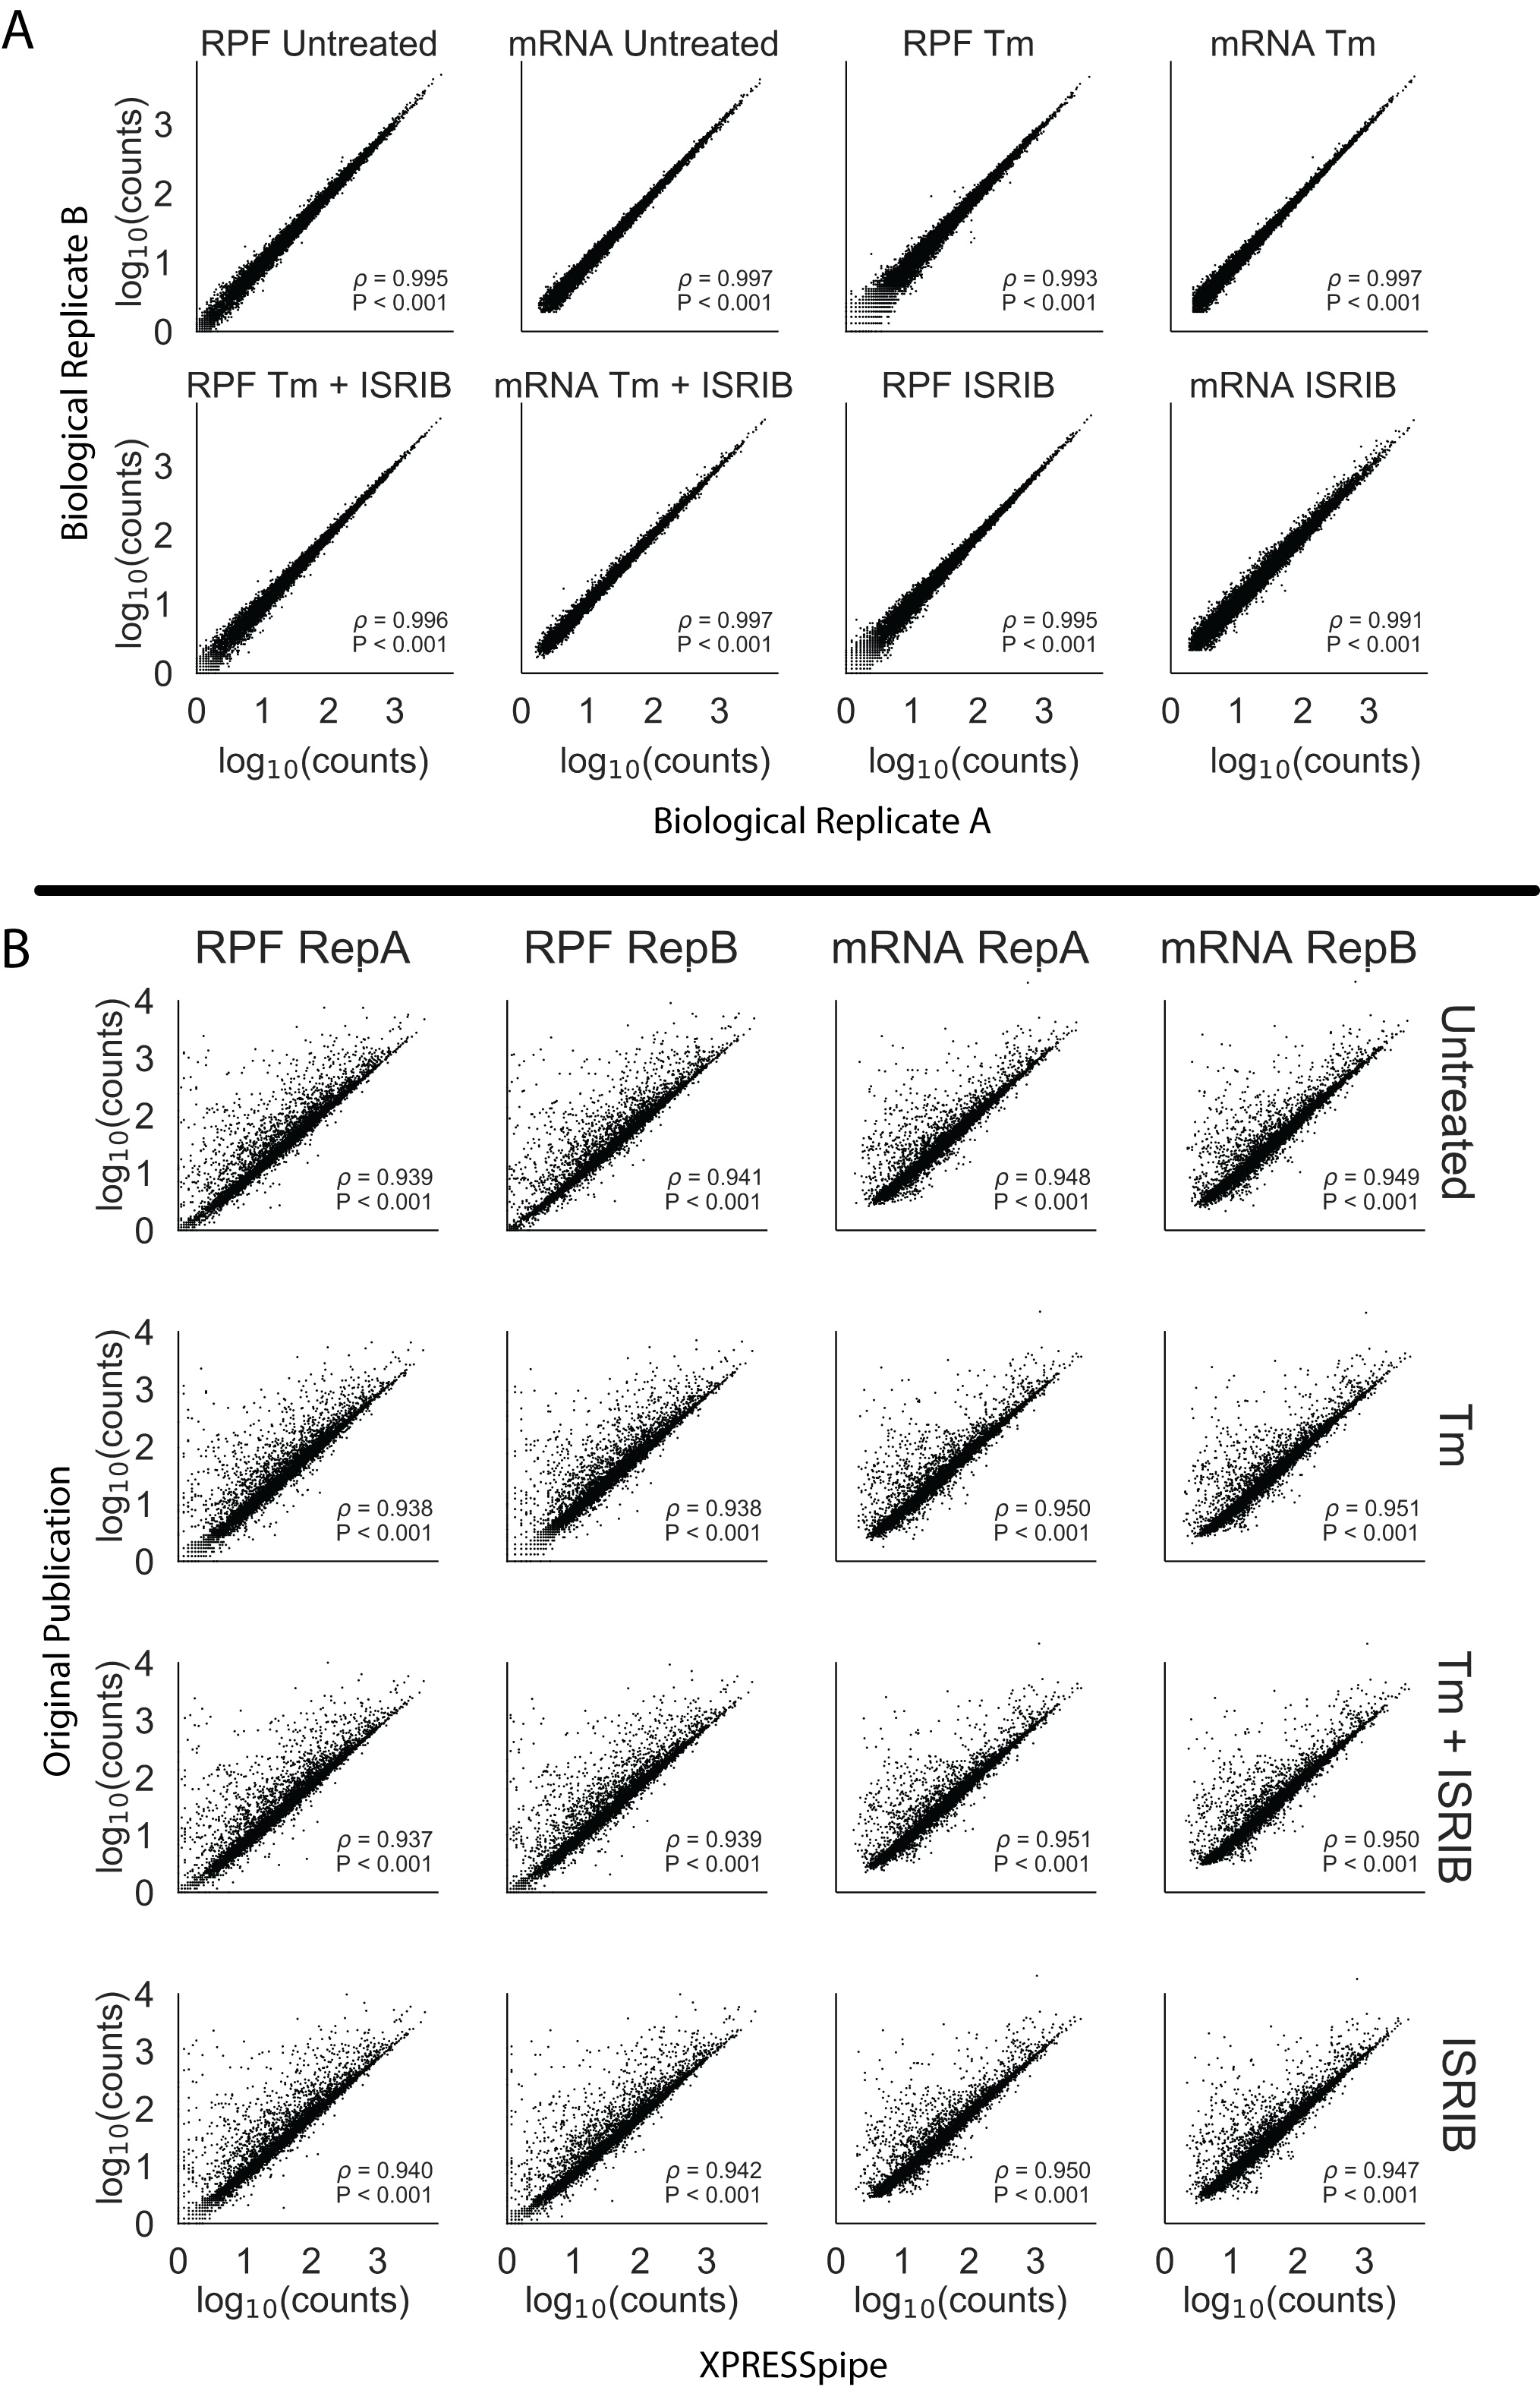
\includegraphics[width=180mm]{figures/xpresspipe_supplement3.png}
  \caption{\textbf{IGV coverage plots for neurologically annotated genes passing strict thresholding.}}
  \label{fig:supplement3}
\end{figure}

\begin{figure}
\centering
  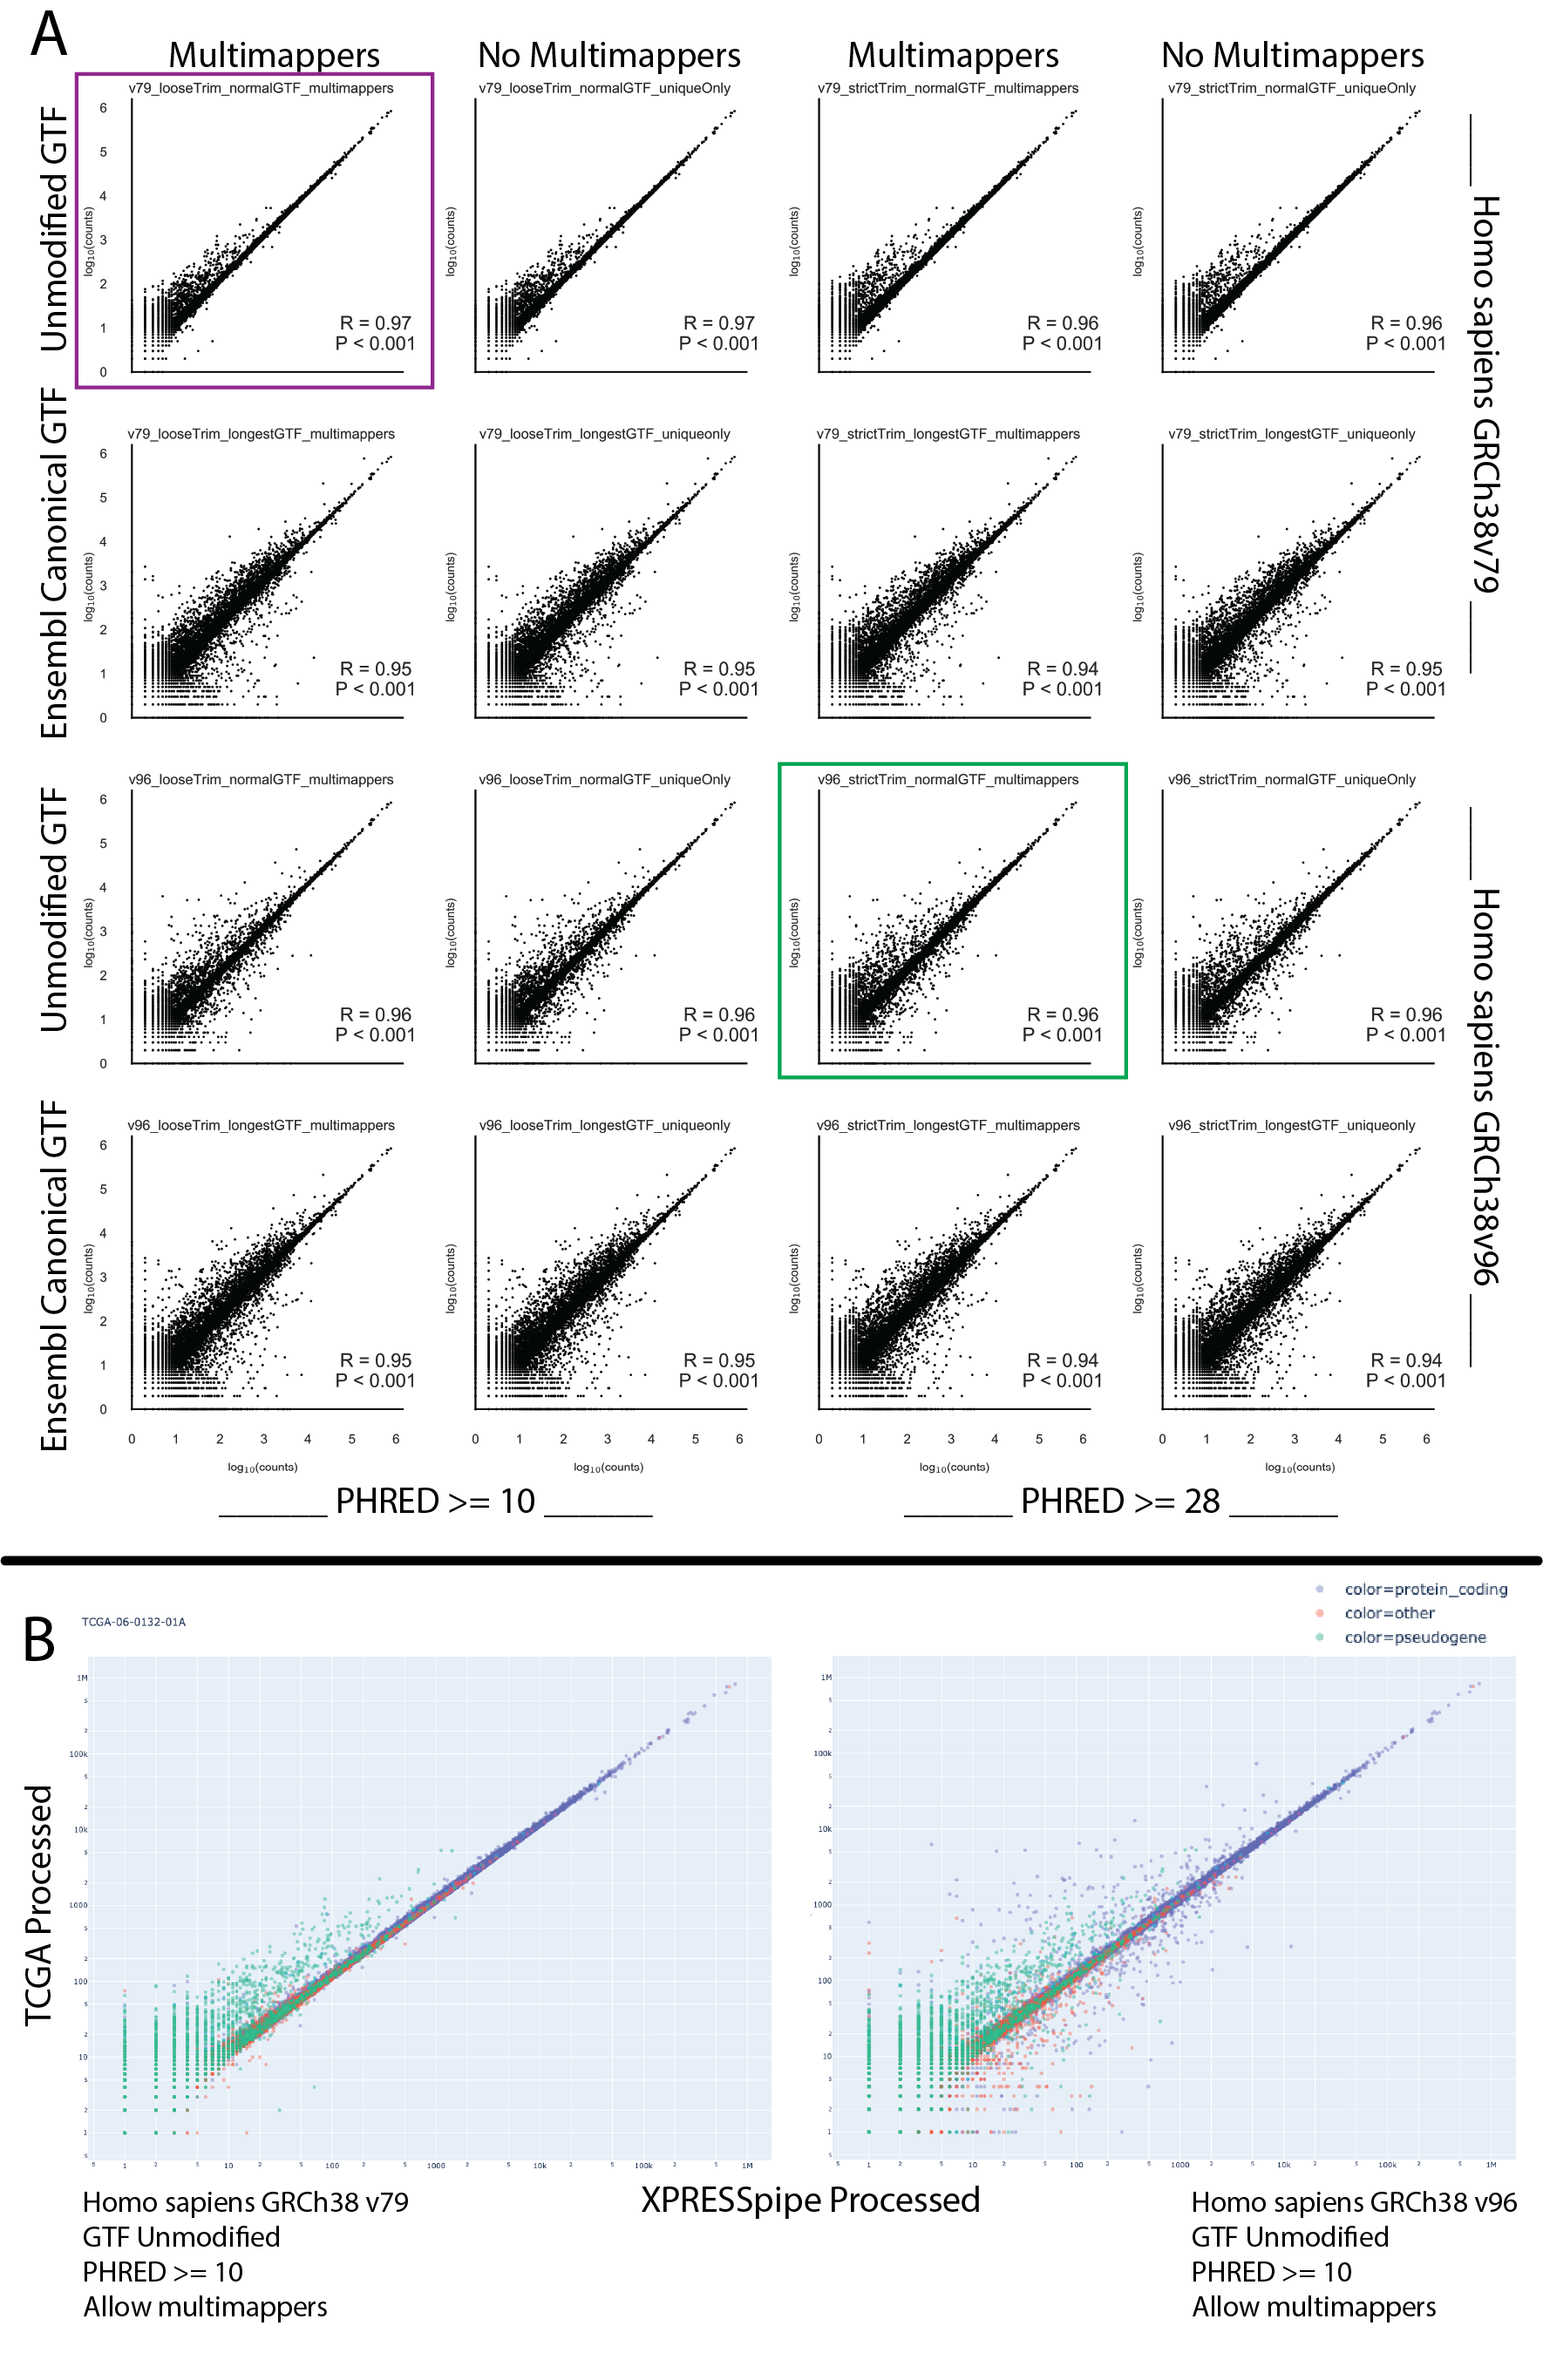
\includegraphics[width=180mm]{figures/xpresspipe_supplement4.png}
  \caption{\textbf{Sample TCGA-06-0132-01A RNA-seq count data compared between TCGA count data and various conformations of the XPRESSpipe pipeline.} A) An overview of how different conformations of the XPRESSpipe peRNAseq pipeline compared to the published TCGA count data. The x-axis data in the plot enclosed in maroon most closely mirrors the settings used in the published TCGA RNA-seq pipeline. The x-axis data in the plot enclosed in green used XPRESSpipe default settings and the most current reference transcriptome at the time of writing. B) An example of the differences arising solely by varying transcriptome reference version. The plot on the left was processed by using GRCh38v79 and the plot of the right was processed using CRCh38v96. Both used un-modified GTF files of the given file version, both allowed multimappers (however HTSeq does not use multimapped reads in quantification, so this does not affect the quantified reads in this case), and used a PHRED threshold greater than or equal to 10. Blue points represent protein-coding genes, green points represent pseudogenes, and orange points represent other genes.}
  \label{fig:supplement4}
\end{figure}


\end{document}
